\chapter{Proposta}
\label{proposta}
\section{Metodologia}

\subsection{Metodologia de pesquisa}

O ser humano, desde os seus primeiros anos de vida até seus últimos dias de vida busca por mais conhecimento de alguma forma, sendo as dúvidas e questionamentos as principais causas para descobrir respostas para essas perguntas \cite{Paschoarelli_Medola_Bonfim_2018}. A pesquisa auxilia o ser humano nessa trajetória de busca por mais conhecimento, para solucionar problemas do mundo real \cite{gil:2008}.

Segundo Gil (\citeyear{gil:2002}), o objetivo de pesquisa se divide em três categorias:

\begin{itemize}
    \item \textbf{Exploratória:} possibilita uma maior familiaridade com o contexto da problemática, com o princípio de aprimorar ideias para a solução;
    
    \item \textbf{Descritiva:} permite a descrição das características de algum determinado fenômeno ou um grupo 
    de seres vivos ou relação entre variáveis;
    
    \item \textbf{Explicativa:} promove a identificação dos fatores que ocasionam ou ajudam para o acontecimento de determinado fenômeno.

\end{itemize}

Conforme Freitas (\citeyear{de2013metodologia}), para a abordagem do problema existem dois tipos:

\begin{itemize}
    \item \textbf{Quantitativo:} considera que tudo pode ser quantificado, isto é, converter informações em números para poder ser classificado e analisado posteriormente, e para isso, é necessário o uso de técnicas estatísticas;
    
    \item \textbf{Qualitativo:} não exige técnicas estatísticas, pois a ideia principal dele é analisar indutivamente os dados, sendo que o processo e seu significado são os pontos de foco;
\end{itemize}


De acordo com Freitas (\citeyear{de2013metodologia}), sobre a natureza da pesquisa, pode ser:

\begin{itemize}
    \item \textbf{Básica:} intuito de produzir novos conhecimentos úteis para o crescimento da ciência, sem ter uma previsão de aplicação prática daquilo;

    \item \textbf{Aplicada:} também tem o objetivo de gerar novos conhecimentos, mas visado para a aplicação prática para a solução de problemas específicos da vida real.
\end{itemize}

Um dos procedimentos de pesquisa que existem é a pesquisa-ação, ela consiste em quando há um interesse coletivo para solucionar um determinado problema, no qual os pesquisadores e os participantes estão envolvidos nesse problema de forma cooperativa ou participativa, com o intuito de solucionar ou no mínimo esclarecer o problema da situação, aumentando o nível de conhecimento dos pesquisadores e dos participantes \cite{de2013metodologia}.

Segundo Thiollent (1997), citado por Costa, Politano e Pereira (\citeyear{Costa}), às etapas da pesquisa-ação são as seguintes:

\begin{itemize}
    \item \textbf{Diagnóstico:} identificar o problema no contexto que o pesquisador tem interesse em resolver;

    \item \textbf{Planejamento da ação:} arquitetar ações alternativas para a solução do problema, melhor dizendo, desenvolver um planejamento de ação;

    \item \textbf{Execução da ação:} aplicação do planejamento da fase anterior com o auxílio de um roteiro;

    \item \textbf{Avaliação da ação:} monitorar as ações implementadas para compreender se os resultados são os esperados.
\end{itemize}

Para este trabalho foi decidido aplicar como objetivo de pesquisa a categoria exploratória, pois como o conhecimento sobre sistema de recomendação não era compreendido ou era superficial, era necessário adquirir mais conhecimento sobre os devidos conceitos, assim sendo, houve um empenho maior em pesquisa bibliográfica para achar conteúdos da área e trabalhos semelhantes. Podendo sempre usar ela quando se deparar com algum conceito desconhecido a fim de entendê-lo melhor \cite{Moretti:2018}.

Para o contexto do presente trabalho foi escolhido a abordagem quantitativa, visto que a ideia principal do mesmo é apresentar resultados de natureza estatística como a métrica CVR (\textit{Conversion Rate}) que será aplicada ao final e abordada mais a frente no trabalho. Com essa métrica será possível medir o grau de melhoria aplicando-se uma abordagem de recomendação comparado com uma já existente em um sistema.

Como o objetivo deste trabalho é desenvolver um produto (sistema de recomendação) para o cliente (Liva) e é necessário buscar mais conhecimento sobre o contexto do problema para solução do mesmo, foi escolhido para a natureza de pesquisa a categoria aplicada.

Para o procedimento de pesquisa foi utilizado a pesquisa bibliográfica no início do trabalho para conhecer os conceitos, abordagens e técnicas de sistema de recomendação.

Para o TCC1 foi realizado as fases de diagnóstico e planejamento e com relação a fase de execução da ação e avaliação dela será executado no TCC2. Para a fase de diagnóstico foi realizado reuniões presenciais e remotas com o gerente de produtos da Liva, Arthur Bersan, sobre levantamento de informações do problema, e houve reuniões presenciais com o orientador Vandor Rissoli sobre questões de pesquisa e objetivos.

A fase com maior duração foi a de planejamento, pois foi realizado uma extensa pesquisa e coleta de referências bibliográficas sobre a área de sistemas de recomendações, para decidir quais abordagens são recomendadas para o contexto do trabalho e pesquisa sobre soluções parecidas, e com isso foi construído o referencial teórico. Além disso, foi efetuado o planejamento da proposta como: a arquitetura, metodologia de desenvolvimento, levantamento de funcionalidades, protótipo de baixa e alta fidelidade e tecnologias.

A execução da ação será a implementação do sistema de recomendação como um serviço a parte dos serviços da \textit{startup} Liva, e como dito antes, será realizada no TCC2, ou seja, será posteriormente mais detalhado em seu decorrer. O mesmo acontece na fase de avaliação, em que a reflexão dos resultados será realizada, para assim, serem apresentados para a banca do TCC2.

\begin{table}[H]
\centering
\setlength{\tabcolsep}{20pt}
\begin{tabular}{cccc}
\hline
\textbf{\begin{tabular}[c]{@{}c@{}}Quanto à\\ abordagem\end{tabular}} & \textbf{\begin{tabular}[c]{@{}c@{}}Quanto ao\\ objetivo\end{tabular}} & \textbf{\begin{tabular}[c]{@{}c@{}}Quanto à\\ natureza\end{tabular}} & \textbf{\begin{tabular}[c]{@{}c@{}}Quanto ao\\ procedimento\end{tabular}} \\ \hline
\begin{tabular}[c]{@{}c@{}}Pesquisa\\ quantitativa\end{tabular} & \begin{tabular}[c]{@{}c@{}}Pesquisa\\ exploratória\end{tabular} & \begin{tabular}[c]{@{}c@{}}Pesquisa\\ aplicada\end{tabular} & \begin{tabular}[c]{@{}c@{}}Pesquisa bibliográfica\\ e Pesquisa-ação\end{tabular} \\ \hline
\end{tabular}
\caption[Escolha de metodologia de pesquisa]{Escolha de metodologia de pesquisa. Fonte: Autor}
\end{table}

\begin{figure}[H]
    \centering
    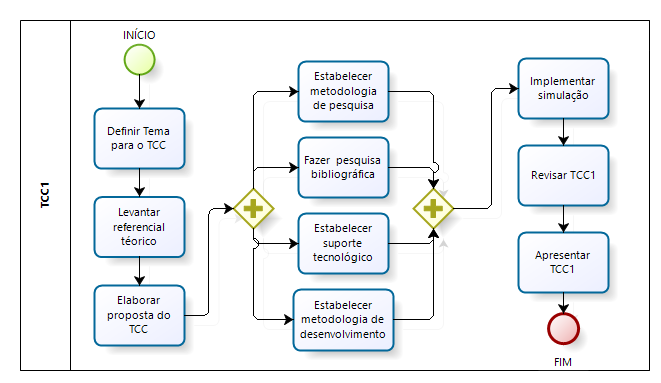
\includegraphics[scale=0.9]{figuras/proposta/fluxo_atividade_tcc1.png}
    \caption[Fluxo de atividades do TCC1]{Fluxo de atividades do TCC1. Fonte: Autor}
    \label{fig:fluxo_atividade_tcc1}
\end{figure}

Cada tarefa do fluxo de atividades do TCC1 (figura \ref{fig:fluxo_atividade_tcc1}) será sucintamente descrito a seguir:

\begin{itemize}
    \item \textbf{Definir Tema para o TCC:} é discutido a área em que será feita o trabalho até chegar em uma decisão final;

    \item \textbf{Levantar referencial teórico inicial:} é estudado de forma introdutória sobre o tema escolhido para averiguar se é possível realizar a proposta do trabalho;

    \item \textbf{Elaborar proposta da monografia:} estabelecer escopo do trabalho, objetivo, questões de pesquisa, justificativa e metodologia a ser usada, podendo haver alterações de acordo com o andamento do trabalho;

    \item \textbf{Estabelecer metodologia de pesquisa:} após o início do estudo do tema selecionado anteriormente, é possível definir quais metodologias de pesquisa serão usadas;

    \item \textbf{Realizar pesquisa bibliográfica:} envolve a pesquisa de artigos, revistas e de trabalhos científicos da mesma área deste trabalho de forma detalhada para servir de fundamento para os objetivos acertados anteriormente;

    \item \textbf{Estabelecer suporte tecnológico:} seleção das tecnologias que serão usadas para o desenvolvimento do trabalho;

    \item \textbf{Estabelecer metodologia de desenvolvimento:} seleção e planejamento da metodologia de desenvolvimento que será utilizada para implementação da proposta;

    \item \textbf{Implementar simulação:} fase de implementação inicial da solução para validação da proposta e identificação de possíveis riscos que possam interferir no desenvolvimento do trabalho;

    \item \textbf{Revisar TCC1:} Revisar todos os tópicos da parte escrita do trabalho para verificar se é necessário alguma correção;

    \item \textbf{Apresentar TCC1:} apresentação do tema para a banca examinadora na Universidade Brasília - campus FGA (Gama) com o intuito de aprimorar a proposta.

\end{itemize}

\begin{figure}[H]
    \centering
    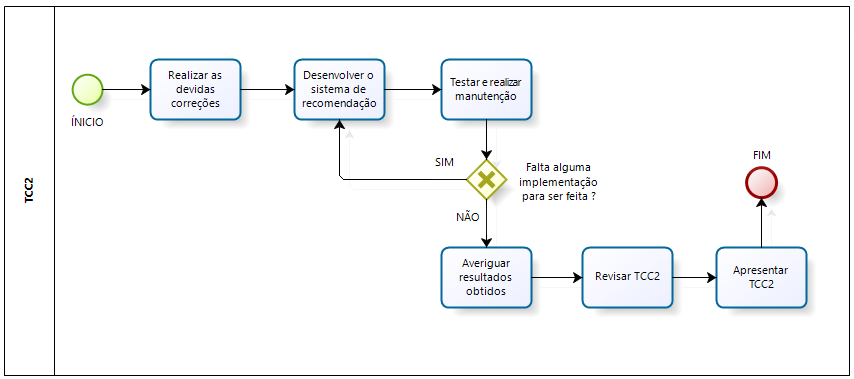
\includegraphics[scale=0.9]{figuras/proposta/fluxo_atividade_tcc2.png}
    \caption[Fluxo de atividades do TCC2]{Fluxo de atividades do TCC2. Fonte: Autor}
    \label{fig:fluxo_atividade_tcc2}
\end{figure}

Na figura \ref{fig:fluxo_atividade_tcc2} pode ser visto o fluxo de tarefas para condução do TCC2 e uma breve descrição de cada tarefa, a seguir:

\begin{itemize}
    \item \textbf{Realizar as devidas correções:} após apresentação para a banca examinadora será feito as devidas correções da monografia;

    \item \textbf{Desenvolver o sistema de recomendação:} implementar o sistema de recomendação usando as três abordagens estudadas (\textit{collaborative filtering, content-based filtering e critic-based filtering}), sendo duas delas feitas com \textit{machine learning}. Será feito a parte de virtualização de ambiente completa, tanto do ambiente de desenvolvimento quanto de produção, a integração contínua e o \textit{deploy} automático;

    \item \textbf{Averiguar resultados obtidos:} será feito a análise dos resultados;
    
    \item \textbf{Revisar TCC2:} verificar se os objetivos do trabalho foram cumpridos como um todo e revisar todos os tópicos da parte escrita da monografia;

    \item \textbf{Apresentar TCC2:} apresentação da parte prática da monografia para a banca examinadora na Universidade Brasília - campus FGA (Gama).
    
\end{itemize}

\subsection{Metodologia de desenvolvimento}

\subsubsection{\textit{Scrum}}

Para o presente trabalho foi escolhido como metodologia de desenvolvimento o \textit{Scrum} que é uma metodologia ágil muito utilizada nos últimos anos pela indústria de desenvolvimento de software, pois esse tipo de  gerenciamento organizacional ágil oferece às organizações de software um nova e dinâmica gestão para não só sobreviver, mas ter sucesso no setor que constantemente há mudanças e inovações \cite{ijcf94}. Outros pontos positivos serão detalhados a seguir.

Essa metodologia é baseada na ideia de que muitos processos no desenvolvimento de software são bem difíceis de serem previstos, sendo assim, a flexibilidade adotada por essa metodologia ágil facilitaria muito mais a implementação das aplicações \cite{ijcf94}.

Como este trabalho é um software que deve ser entregue com uma alta qualidade esperada pelos superiores da Liva, e deve ser colocado que imprevistos são bem prováveis de acontecer, além de mudanças ao decorrer do trabalho, é necessário empregar um \textit{framework} que atenda a essas características, ou seja, uma metodologia onde é permitido entregar subconjuntos do projeto a cada período de tempo e que possa ser melhorado no andamento do desenvolvimento junto com um \textit{feedback} contínuo.

O princípio do \textit{Scrum} é entregar produtos de alta qualidade, após vários períodos de desenvolvimento chamados de \textit{Sprints} que tem duração entre duas e quatro semanas, mas para esse trabalho terá a duração de 2 semanas. Em cada início de um ciclo será realizado uma reunião chamada de \textit{Sprint Planning}, na qual é feito o planejamento do que será implementado e entregue ao cliente. Da segunda \textit{Sprint} em diante é realizado uma outra reunião chamada de \textit{Sprint Review} que seria a revisão do ciclo passado com o propósito de rever o que foi feito na \textit{Sprint} antes de realizar o \textit{Sprint Planning} \cite{ijcf94}.

Como instrumento para organização do que é necessário fazer, será feito o \textit{Product Backlog}, que é uma lista com todas as funcionalidades que devem conter com base nos requisitos levantados através do cliente. Cada funcionalidade será agrupada pelo seu nível de prioridade. Essa lista é dinâmica e será atualizada de acordo com o andamento do projeto, identificando mais necessidades, como correções e melhorias.

A lista de funcionalidades que é planejada para ser feita no período da \textit{Sprint} é chamada de \textit{Sprint Backlog} , sendo recomendado possuir pelo menos uma melhoria de alta prioridade ao cliente que foi identificada anteriormente \cite{ijcf94}.

Cada funcionalidade do \textit{Product Backlog} será descrito como \textit{User Story} (estória de usuário), na qual é uma representação de cada necessidade do cliente sob seu ponto de vista \cite{knowledge21:2019}.

\subsubsection{Kanban}

Kanban (cartão) será uma outra metodologia ágil utilizada no presente projeto. Ele é muito utilizada ao lado do \textit{Scrum}, sendo um sistema visual para controlar a gestão de atividades em um processo. Ela tem o intuito de controlar o fluxo de trabalho, balancear a ordem dos processos e respeitar a produtividade da equipe \cite{ARTIA:2019}.

O Kanban é divido em três colunas: \textit{to do, doing e done}, mas é possível colocar mais colunas caso seja desejado, para assim, ficar mais relacionado ao contexto do processo. Para o presente trabalho haverá seis colunas: \textit{Product Backlog, Sprint Backlog, Doing, Testing, Review} e \textit{Done}. Para cada coluna há \textit{cards} que representam uma atividade que está em uma dessas respectivas fases do processo. De acordo com o andamento, os \textit{cards} serão movidos para as fases seguintes \cite{ARTIA:2019}.

Para realização dessa metodologia será utilizado a ferramenta ZenHub \cite{zenhub:2019}.

\subsubsection{\textit{Product Backlog} inicial}

Para obter um conhecimento inicial sobre o projeto, foi levantado as seguintes \textit{features, user stories} e \textit{technical stories}:

\begin{itemize}
    \item \textit{Features}:
    \begin{itemize}
        \item \textbf{FE01 - Recomendador baseado em crítica:} possibilitará o usuário receber recomendações de imóveis baseadas em críticas sobre características de imóveis, feitas por ele;

        \item \textbf{FE02 - Recomendador baseado em \textit{machine learning}:} permitirá o usuário receber recomendações de imóveis baseado nas ações dele no site;
    \end{itemize}
    
    \item \textit{User stories}:
    \begin{itemize}
        \item \textbf{FE01US01 - Visualizar perfil de busca:} eu, como usuário, desejo visualizar meu perfil de busca para ter conhecimento de como está configurado;
        
        \item \textbf{FE01US02 - Alterar perfil de busca:} eu, como usuário, desejo alterar meu perfil de busca para o ajustar minha preferência e receber recomendações mais precisas;
        
        \item \textbf{FE01US03 - Visualizar recomendações na página principal:} eu, como usuário, desejo visualizar os imóveis recomendados com base nas minhas preferências configuradas no perfil de busca;
        
        \item \textbf{FE01US04 - Criticar características da propriedade:} eu, como usuário, desejo criticar as características de um ou vários imóveis para ter recomendações de imóveis mais precisas com o que eu desejo;
        
        \item \textbf{FE02US05 - Visualizar recomendações na página do imóvel:} eu, como usuário, desejo visualizar recomendações de imóveis baseadas nas minhas ações no site na página de detalhes do imóvel para diminuir o tempo de procura do imóvel ideal para mim;
    \end{itemize}
    
    \item \textit{Technical stories}:
    \begin{itemize}
        \item \textbf{FE02TS01 - Registrar ações do usuário no site:} eu, como desenvolvedor, desejo registrar as ações do usuário no site para poder predizer quais são os imóveis mais prováveis dele gostar.
    \end{itemize}
\end{itemize}

\subsubsection{Papéis}

\textbf{\textit{Product Owner}}. É responsável por potencializar o retorno sobre o ROI (\textit{Return over Investment}), e para isso é necessário que esse papel identifique as características do produto, decidindo quais são as funcionalidades com mais prioridades, criando uma lista ordenada com base na prioridade para a próxima \textit{Sprint} e re-priorizando e refinando continuamente essa lista. De forma resumida, o \textit{Product Owner} é responsável pelos lucros e perdas do produto \cite{Sutherland}.

Esse papel será desempenhado pelo gerente de produtos da Liva, Arthur Bersan, pois ele tem a visão de produto deste trabalho que está sendo desenvolvido, além de também ter conhecimento de engenharia de software.

\textbf{\textit{Scrum Master}}. Tem como atividades ensinar o \textit{Scrum} para o time do produto e aplicá-lo de fato. Seu objetivo principal é ajudar a equipe a alcançar o sucesso, protegendo-os de possíveis interferências externas. Além disso, ele também educa e  orienta o \textit{Product Owner} e a todos do grupo no uso da metodologia ágil. Quando necessário, ajuda a liderar a organização nas difíceis mudanças fundamentais para o sucesso do desenvolvimento ágil \cite{Sutherland}.
	
Quem irá desempenhar esse papel será o professor e orientador Vandor Rissoli, por ser quem vai acompanhar e auxiliar o andamento do trabalho.

\textbf{Time desenvolvimento}. Serão as pessoas que farão a implementação do produto, fazendo entregas a cada \textit{Sprint} \cite{Sutherland}. Esses papéis serão desempenhados pelos orientados Daniel Marques Rangel e Bruno Matias Casas, por possuírem conhecimento técnico sobre as tecnologias, metodologias e contexto do trabalho.

\subsubsection{Fluxo de desenvolvimento}

\begin{figure}[H]
    \centering
    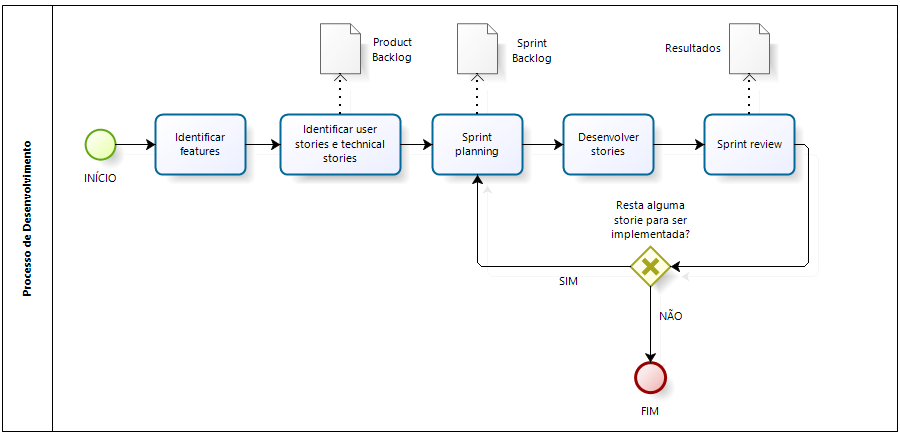
\includegraphics[scale=0.6]{figuras/proposta/fluxo_scrum.png}
    \caption[Fluxo de desenvolvimento do trabalho]{Fluxo de desenvolvimento do trabalho. Fonte: Autor}
    \label{fig:fluxo_scrum}
\end{figure}

\begin{itemize}
    \item \textbf{Identificar features:} averiguar quais são os módulos de requisitos do projeto existentes.
    
    \item \textbf{Identificar \textit{user stories} e \textit{technical stories}:} identificar as histórias de cada \textit{feature} definida anteriormente e prioriza-las com o nível de importância para o cliente;
    
    \item \textbf{\textit{Sprint planning}:} planejar quais histórias serão desenvolvidas na \textit{Sprint}, sendo seguido a ordem de prioridade descrita no \textit{product backlog};
    
    \item \textbf{Desenvolver stories:} implementar e testar as histórias descritas no \textit{Sprint backlog} até a conclusão dela;
    
    \item \textbf{\textit{Sprint review}:} verificar quais \textit{stories} foram realmente feitas e quais estão pendentes e se houve a necessidade de criar novas, seja \textit{user} ou \textit{technical stories}.
\end{itemize}

\section{Cronograma}

Foi planejado dois cronogramas para serem seguidos no TCC1 e no TCC2 com intuito de dividir as atividades durante o semestre. O primeiro cronograma é referente a primeira parte do projeto que abrange todas as atividades referentes ao TCC1 e o segundo cronograma é referente as atividades que foram propostas para o TCC2. A utilização do cronograma se faz necessária para ter um gerenciamento de tempo das atividades que precisam ser realizadas para a conclusão deste trabalho.

\begin{table}[H]
\centering
\begin{tabular}{lccccc}
\hline
\textbf{} & \textbf{Ago} & \textbf{Set} & \textbf{Ou} & \textbf{Nov} & \textbf{Dez} \\ \hline
Escrever monografia & X & X & X & X &  \\ \hline
Estudo inicial do tema & X &  &  &  &  \\ \hline
Definir de escopo e objetivo & X &  &  &  &  \\ \hline
Desenvolver proposta &  & X & X &  &  \\ \hline
Determinar metodologias &  &  & X &  &  \\ \hline
Revisar TCC1 &  &  & X & X &  \\ \hline
Apresentar TCC1 &  &  &  &  & X \\ \hline
\end{tabular}
\caption[Cronograma do TCC1]{Cronograma do TCC1. Fonte: Autor}
\end{table}

\begin{table}[H]
\centering
\begin{tabular}{lccccc}
\hline
\textbf{} & \textbf{Mar} & \textbf{Abr} & \textbf{Mai} & \textbf{Jun} & \textbf{Jul} \\ \hline
Efetuar revisão da banca & X &  &  &  &  \\ \hline
Implementar proposta & X & X & X & X &  \\ \hline
Analisar resultados obtidos &  &  &  & X & X \\ \hline
Apresentar TCC2 &  &  &  &  & X \\ \hline
\end{tabular}
\caption[Cronograma do TCC2]{Cronograma do TCC2. Fonte: Autor}
\end{table}

\section{Sistema de recomendação}

\subsection{Visão geral}

O sistema proposto consiste de um novo sistema de recomendação para a plataforma Web Liva.vc. Esse sistema de recomendação seguirá duas abordagens: sistema de recomendação baseado em crítica (\ref{Critiquing-based}) e sistema de recomendação baseado em \textit{machine learning} (\ref{machineLearning}). Por se tratar do uso de duas abordagens, isso faz com que se torne um sistema de recomendação híbrido (\ref{Hybrid}). Para fazer a combinação dessas duas abordagens é utilizada a técnica de hibridação \textit{mixed}, que como já abordado, refere-se a recomendações de diferentes recomendadores que são apresentadas juntas.

Dito isto o sistema proposto irá combinar essas duas abordagens que irão englobar diferentes páginas do site da Liva. Existem duas principais páginas que irão ser atualizadas para o novo sistema de recomendação: página principal do cliente (Figura \ref{fig:pagina_principal}) e página de detalhes de uma propriedade (Figura \ref{fig:pagina_detalhes})

\begin{figure}[H]
    \centering
    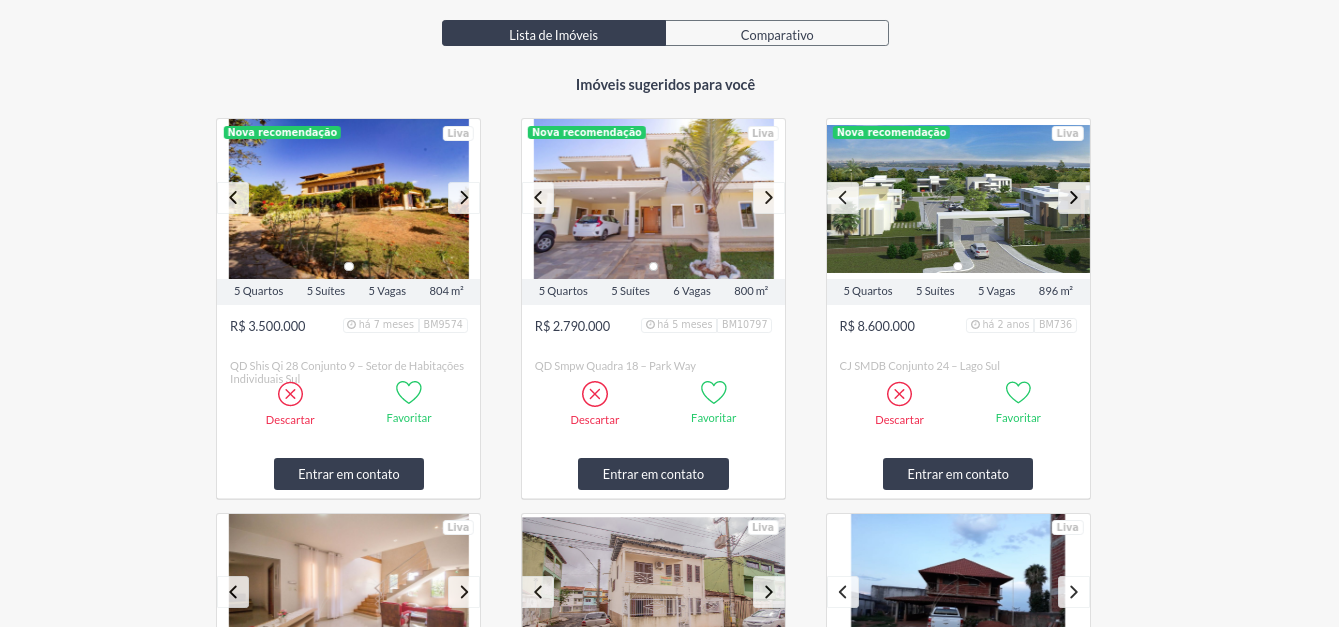
\includegraphics[scale=0.33]{figuras/proposta/pagina_principal.png}
    \caption[Página principal do cliente]{Página principal do cliente. Fonte: (LIVA.VC, 2019)}
    \label{fig:pagina_principal}
\end{figure}

\begin{figure}[H]
    \centering
    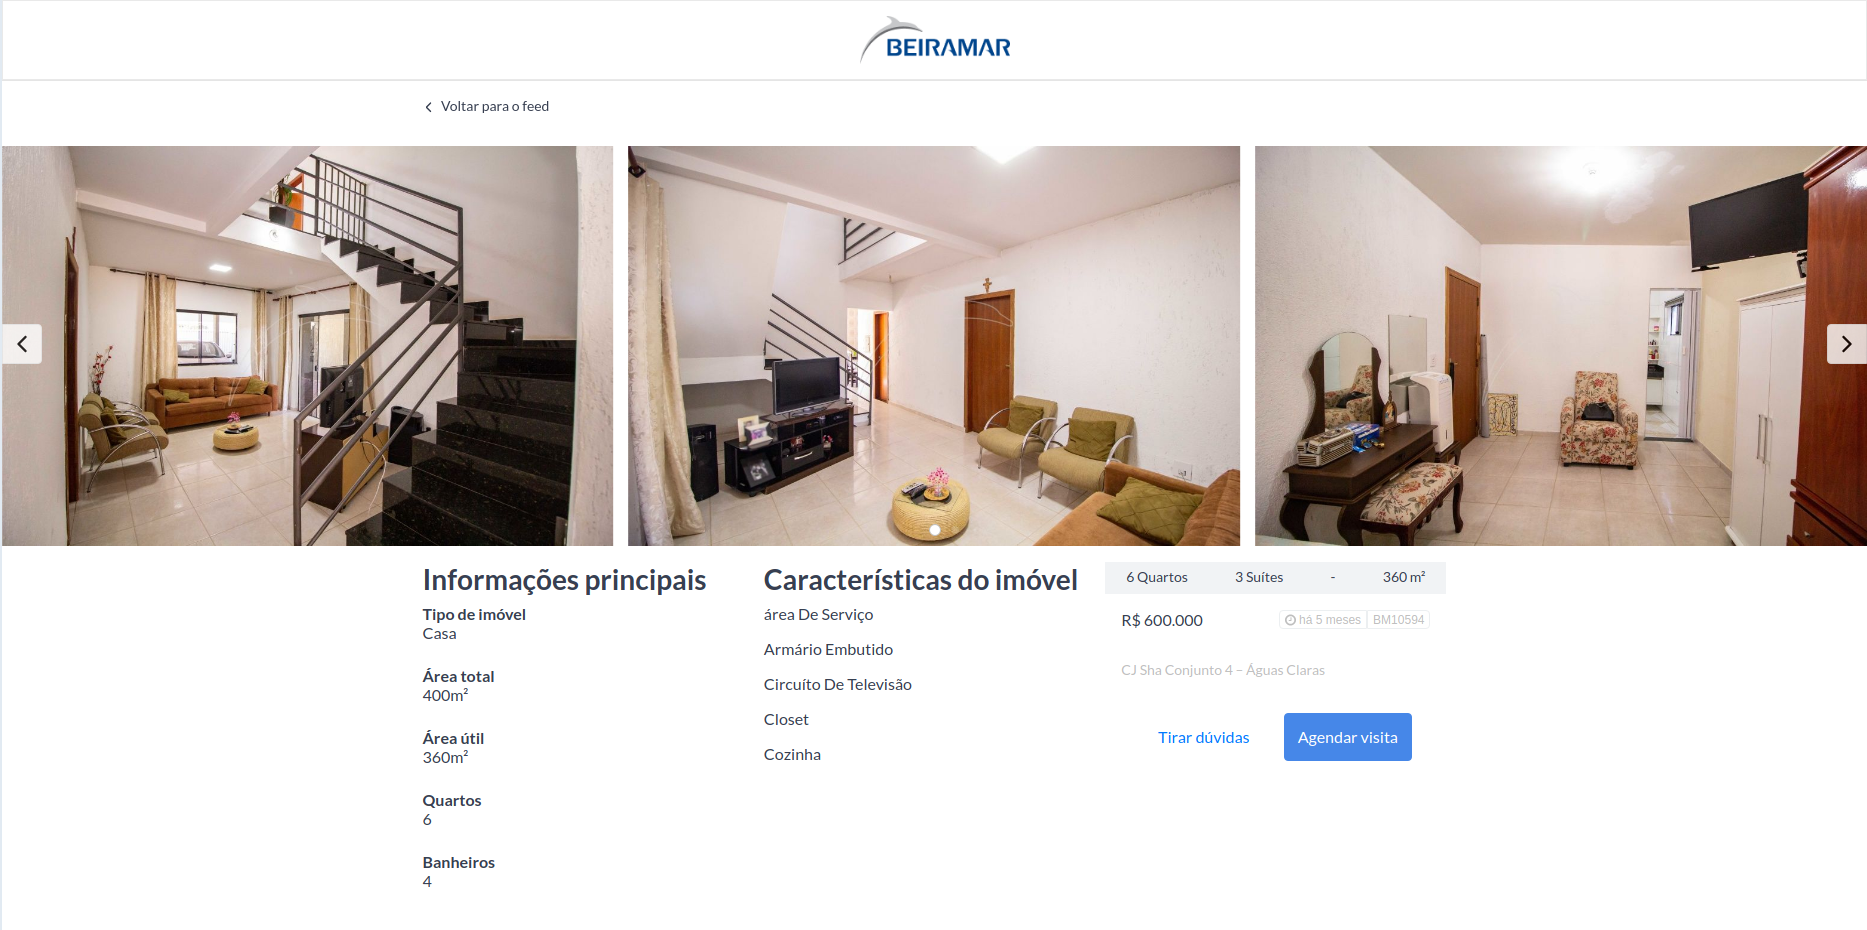
\includegraphics[scale=0.23]{figuras/proposta/pagina_detalhes.png}
    \caption[Página de detalhes da propriedade]{Página de detalhes da propriedade. Fonte: (LIVA.VC, 2019)}
    \label{fig:pagina_detalhes}
\end{figure}

Na página principal existe uma ferramenta de busca denominada “Perfil de Busca” e pode ser acessada por uma modal, como na figura \ref{fig:filtro_busca}.

\begin{figure}[H]
    \centering
    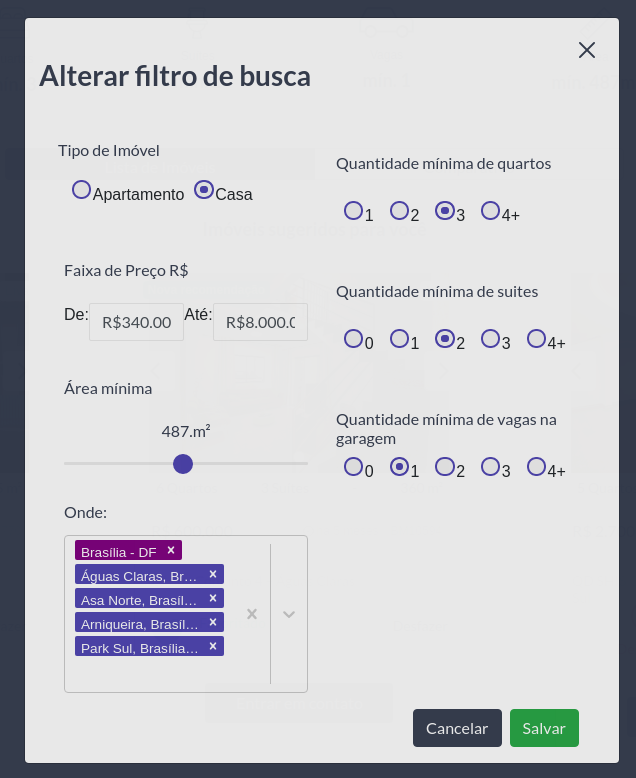
\includegraphics[scale=0.6]{figuras/proposta/filtro_busca.png}
    \caption[Filtro de busca]{Filtro de busca. Fonte: (LIVA.VC, 2019)}
    \label{fig:filtro_busca}
\end{figure}

Aproveitando-se dessa ferramenta de busca para implementação do sistema de recomendação baseado em crítica, será necessário alguns ajustes. Primeiramente serão colocados novos campos para determinar a importância de cada característica de preferência do usuário. Além disso será adicionado um novo campo de quantidade referente a número de banheiros. Os campos que representam a quantidade das características serão alterados para quantidades fixas e não mínimas. A localidade irá se referir somente a um bairro. Essas alterações podem ser vista no protótipo realizado representado na figura \ref{fig:prototipo_search_profile}.

\begin{figure}[H]
    \centering
    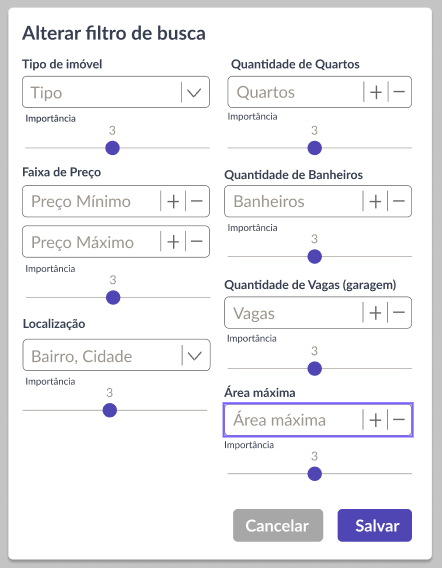
\includegraphics[scale=0.6]{figuras/proposta/prototipo_search_profile.png}
    \caption[Protótipo do filtro de busca]{Protótipo do filtro de busca. Fonte: Autor}
    \label{fig:prototipo_search_profile}
\end{figure}

Ainda na página principal é possível observar a existem de um \textit{feed}, em que se encontram as recomendações do atual recomendador da Liva. Esse \textit{feed} servirá para visualização das recomendações do recomendador baseado em crítica.

A página de detalhes de uma propriedade é acessível por meio de um clique em sua imagem no \textit{feed} da página principal. Nela é possível visualizar todas as características da propriedade. Além disso é possível entrar em contato com o corretor de duas diferentes formas: pedindo mais informações da propriedade e agendando uma visita. Para o recomendador baseado em crítica, será atualizado o componente de visualização de características da propriedade para que possam ser feitas críticas pelo usuário em cima dessas características. Esse novo componente de crítica pode ser observado pelos protótipos apresentados pelas figuras \ref{fig:prototipo_critico1}, \ref{fig:prototipo_critico2}, \ref{fig:prototipo_critico3} e \ref{fig:prototipo_critico4}

\begin{figure}[H]
    \centering
    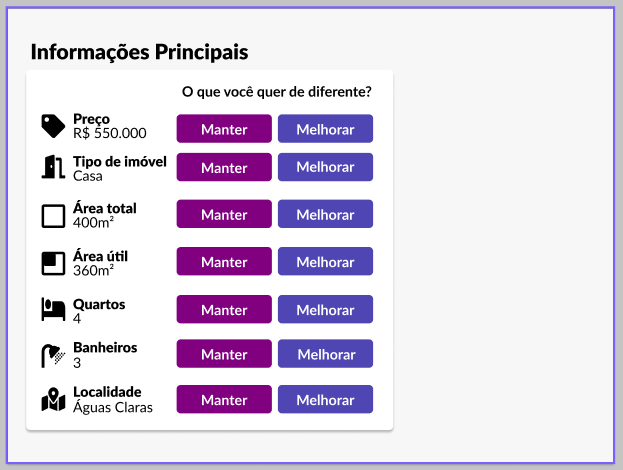
\includegraphics[scale=0.7]{figuras/proposta/prototipo_critico1.png}
    \caption[Detalhes do imóvel com menu de crítica parte 1]{Detalhes do imóvel com menu de crítica parte 1. Fonte: Autor}
    \label{fig:prototipo_critico1}
\end{figure}

\begin{figure}[H]
    \centering
    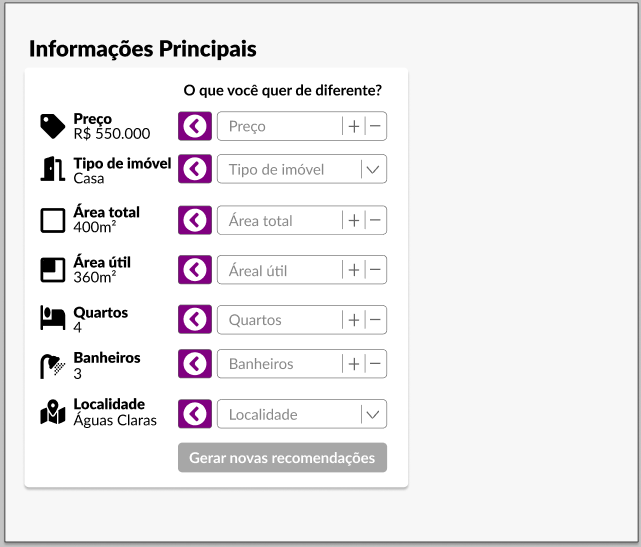
\includegraphics[scale=0.8]{figuras/proposta/prototipo_critico2.png}
    \caption[Detalhes do imóvel com menu de crítica parte 2]{Detalhes do imóvel com menu de crítica parte 2. Fonte: Autor}
    \label{fig:prototipo_critico2}
\end{figure}

\begin{figure}[H]
    \centering
    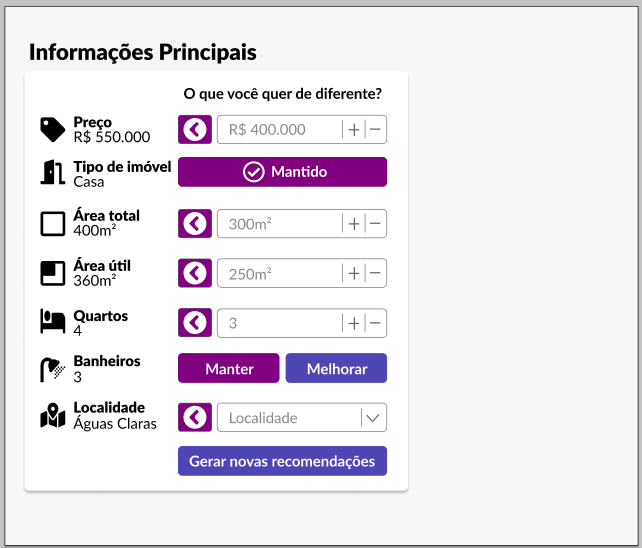
\includegraphics[scale=0.8]{figuras/proposta/prototipo_critico3.png}
    \caption[Detalhes do imóvel com menu de crítica parte 3]{Detalhes do imóvel com menu de crítica parte 3. Fonte: Autor}
    \label{fig:prototipo_critico3}
\end{figure}

\begin{figure}[H]
    \centering
    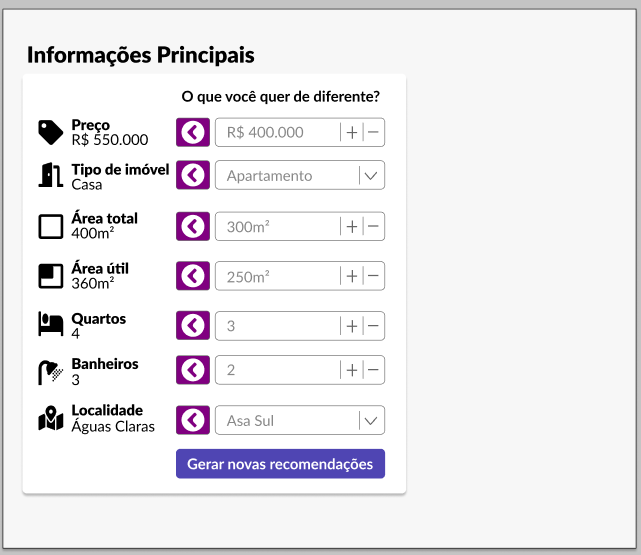
\includegraphics[scale=0.8]{figuras/proposta/prototipo_critico4.png}
    \caption[Detalhes do imóvel com menu de crítica parte 4]{Detalhes do imóvel com menu de crítica parte 4. Fonte: Autor}
    \label{fig:prototipo_critico4}
\end{figure}

O usuário poderá criticar uma propriedade escolhendo entre manter e mudar os valores para cada característica. Após as críticas serem atribuídas as características de uma propriedade seu perfil de busca é refinado, dessa forma gerando novas recomendações no \textit{feed} da página principal.

Ainda referente a página de detalhes, será adicionado um novo componente na lateral direita para a visualização das recomendações do módulo de \textit{machine learning}. Esse componente será a representação de cinco propriedades contendo todas suas características principais. Esse componente é representado pelo protótipo na Figura \ref{fig:prototipo_recommender_system}.

\begin{figure}[H]
    \centering
    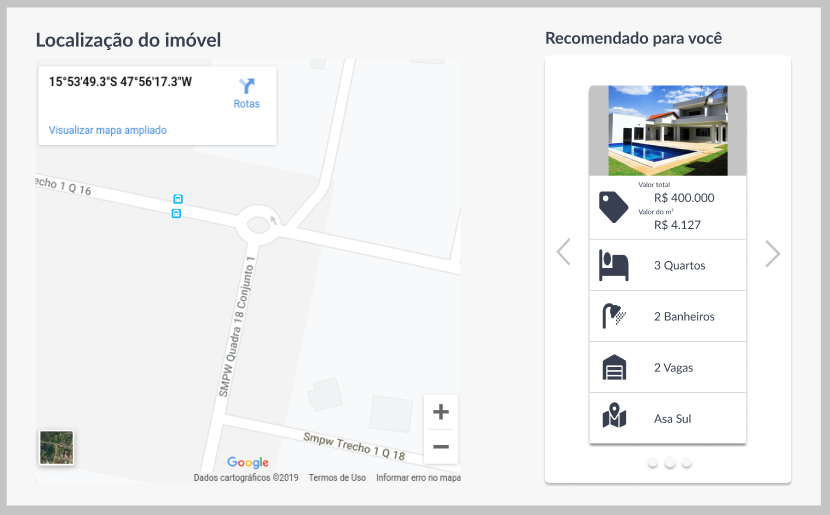
\includegraphics[scale=0.53]{figuras/proposta/prototipo_recommender_system.png}
    \caption[Protótipo do carrossel de recomendações]{Protótipo do carrossel de recomendações. Fonte: Autor}
    \label{fig:prototipo_recommender_system}
\end{figure}

O recomendador do módulo de \textit{machine learning} terá como dados de entrada registros de ações de usuários na plataforma, como: cliques ou descartes em propriedades no \textit{feed}, alterações no perfil de busca e até mesmo em requisições de contato com o cliente. Dessa forma as recomendações serão realizadas em tempo-real no momento em que um usuário entra na página de detalhes de uma propriedade.

\subsection{Arquitetura}

Para este trabalho de conclusão de curso, será desenvolvido uma aplicação web como um serviço de sistema de recomendação para o site Liva.vc. Sua principal funcionalidade é fornecer recomendações de propriedades para usuários clientes de imobiliárias vinculadas a Liva.

Para apresentar a arquitetura do projeto, houve uma divisão em três níveis, em que serão apresentadas as características e os motivos de suas implementações. Começando com o primeiro nível uma visão mais generalizada do sistema é apresentada. Em seguida serão apresentadas características ainda mais detalhadas nos seguintes níveis. 

\subsubsection{Nível 1}

Considerando o sistema de recomendação como uma caixa preta, a figura \ref{fig:sr_nivel1} demonstra a interação da Liva com o sistema de recomendação, descrevendo suas entradas e saídas de dados.

\begin{figure}[H]
    \centering
    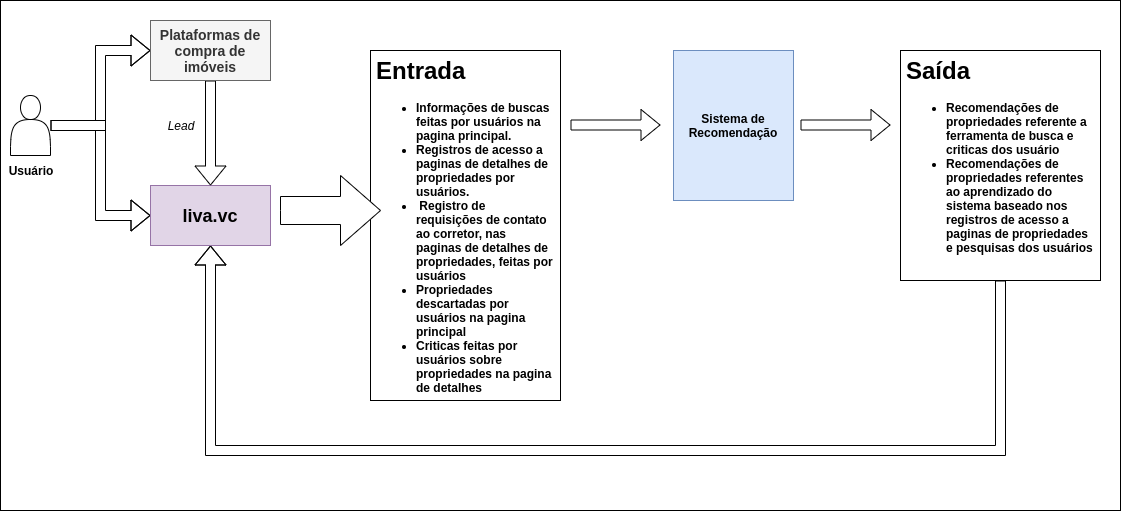
\includegraphics[scale=0.4]{figuras/proposta/sr_nivel1.png}
    \caption[Sistema de recomendação como caixa preta]{Sistema de recomendação como caixa preta. Fonte: Autor}
    \label{fig:sr_nivel1}
\end{figure}

Como descrito anteriormente, para usuários terem acesso a Liva, eles devem primeiramente ter interagido com uma outra plataforma de vendas de imóveis tais como Zap Imóveis ou Olx. Essa interação refere-se a um \textit{lead}, que é uma requisição de informações  a um corretor a respeito de um imóvel de uma imobiliária vinculada a Liva. Quando usuários acessam a Liva pela primeira vez eles já possuem um Perfil de Busca pré configurado advindo de seu primeiro \textit{lead}. Com isso, logo no primeiro acesso à página principal o usuário já tem os dados de entrada necessários para receber recomendações. A partir desse momento dados de navegação relevantes começam a ser registrados, tais como: trocar seu Perfil de Busca, clicar para visualizar propriedades, descartar propriedades, requisitar contato com o corretor (agendar visita ou pedir informações da propriedade) e criticar características das propriedades. Todo novo registro é enviado ao sistema de recomendação que por sua vez apresentará novas recomendações. Dessa forma a cada novo registro as recomendações são reprocessadas e tornam-se eventualmente mais precisas.

O motivo de se criar um sistema de recomendação baseando-se em dados do processo de consulta do usuário para encontrar uma propriedade adequada, é justificado por eles serem valiosos representantes de sua preferência. Normalmente um usuário consulta diversas vezes e lê várias páginas antes de encontrar a propriedade certa. Esse processo é considerado muito trabalhoso e pode gerar frustrações aos usuários a ponto de fazer-los desistirem. O foco é melhorar a experiência do usuário no sistema durante esse processo, gerando recomendações ainda mais precisas a cada nova interação.

\subsubsection{Nível 2}

Diminuindo ainda mais o nível de abstração da arquitetura, a figura \ref{fig:sr_nivel2} apresenta os sistemas existentes, suas tecnologias e interações do projeto.

\begin{figure}[H]
    \centering
    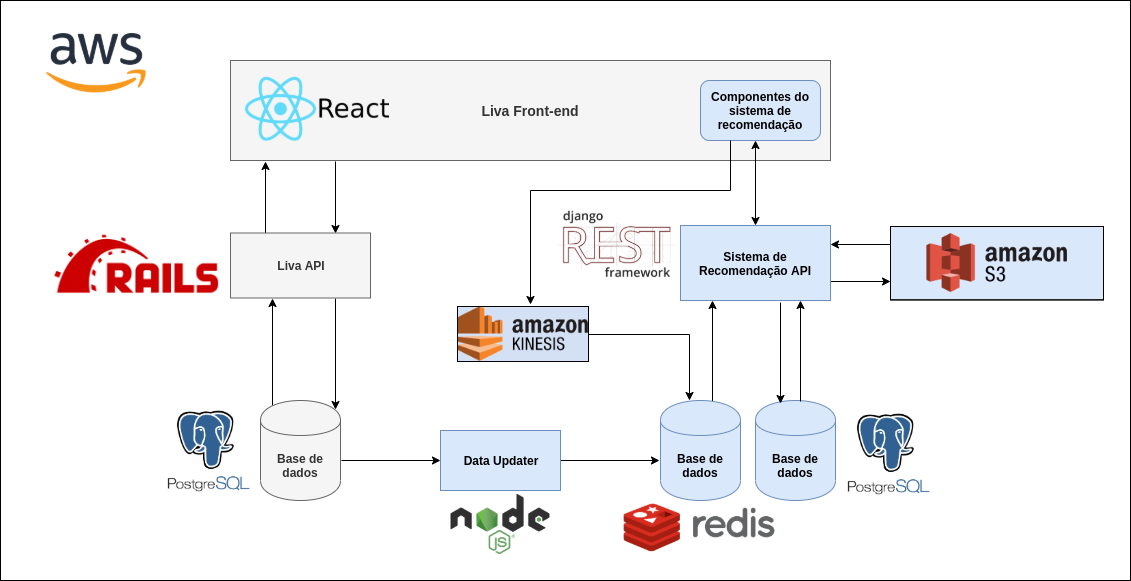
\includegraphics[scale=0.4]{figuras/proposta/sr_nivel2.png}
    \caption[Arquitetura por serviços]{Arquitetura por serviços. Fonte: Autor}
    \label{fig:sr_nivel2}
\end{figure}

A arquitetura existente no sistema da Liva segue o estilo arquitetural Cliente-Servidor, com uma abordagem monolítica. Seu cliente é desenvolvido na linguagem javaScript e com o \textit{framework} React. Sua API na linguagem Ruby com suporte do \textit{framework} Ruby on Rails, integrado a um sistema gerenciador de banco de dados PostgreSQL.

A fim de desenvolver um sistema como um serviço que possa ser utilizado pela Liva sem interferir diretamente em sua estrutura, será implantado uma arquitetura em que o sistema de recomendação a ser implementado é separado do restante do sistema, como demonstrado na Figura \ref{fig:sr_nivel2}, destacado em azul. O sistema é composto por um cliente que é representado pelos novos componentes de interface atribuídos ao \textit{front-end} da Liva. Esses componentes são: nova ferramenta de busca com o componente de importância para cada atributo (Figura \ref{fig:filtro_busca}), componente de crítica (Figura \ref{fig:prototipo_critico1}) e por fim o componente de recomendação, responsável por listar recomendações advindas do módulo de \textit{machine learning} (Figura \ref{fig:prototipo_recommender_system}). Eles se comunicarão através do protocolo HTTP com a API de recomendação e com a tecnologia Amazon Kinesis, que transmitirá dados para o Redis em tempo real.

A API de recomendação será desenvolvida em python com o \textit{framework} Django REST e se comunicará com outras três tecnologias: Redis, PostgreSQL e Amazon S3. A escolha dessa tecnologia foi feita pelo fato de que existem diversas bibliotecas e \textit{framework} desenvolvidos em python que dão suporte para suprir todos os requisitos do sistema a ser desenvolvido, como por exemplo, o XGboost, Scikit-Learn, Numpy, Pandas e o Pickle para solução do módulo de \textit{machine learning}, além do Django REST que possibilita o desenvolvimento de uma API REST.

Como haverá novos componentes na interface gráfica referentes ao sistema de recomendação, eles serão desenvolvidos na linguagem javaScript com o suporte do \textit{framework} React já utilizado na Liva, consequentemente sendo facilmente integrável.

O sistema proposto é composto por um banco de dados de grande escala para o armazenamento de registros dos usuários e propriedades em memória RAM (Redis) para otimização no tempo de respostas de requisições a respeito da recomendação. Além disso há a existência de um banco relacional para backup dos dados e para salvar novos dados de treinos do modelo de \textit{machine learning} (PostgreSQL). O Redis foi escolhido para esse propósito por ser rápido e por ser um banco de dados de valor-chave, o que facilita no mapeamento dos dados. Essas escolhas são essenciais para o sistema de recomendação pois as recomendações das propriedades precisam ser geradas rapidamente para o usuário. Segundo Li et al. \cite{Summo:2017} na plataforma Suumo.jp eles calculam de dez a vinte segundos para um usuário ler as informações da propriedade para somente em seguida visualizarem as recomendações na página de detalhes. 

O Amazon S3 servirá para guardar os dados de treino e o modelo treinado do módulo de \textit{machine learning}. Essa tecnologia é utilizada para melhorar no tempo de treino do modelo, que será feito em lotes, e a fácil distribuição do modelo.

O sistema também é composto por um serviço de \textit{upload} de dados (\textit{Data Updater}), que será desenvolvido na linguagem javascript com o ambiente de execução nodeJS, capaz de ler o banco de dados da Liva e atualizar o banco do sistema de recomendação. Esses dados são basicamente referentes a propriedades.

O sistema de recomendação e todos os serviços que o envolvem serão implantados em ambiente de produção por meio de \textit{containers}, possibilitado pela tecnologia Docker e serão orquestrados pelo serviço do AWS, Amazon ECS, já utilizado na Liva.
	
\subsubsection{Nível 3}
\label{nivel3}
O sistema de recomendação a ser desenvolvido foi dividido em dois módulos. Cada módulo refere-se a um tipo diferente de solução para recomendar itens. Como apresentado anteriormente, o sistema recomendará propriedades para os usuários na página principal do site da Liva, no denominado \textit{feed}, baseado na ferramenta de busca, o Perfil de Busca, e as críticas feitas sobre as propriedades pelos usuários. Essa solução refere-se a técnica \textit{exemple-critiquing} como apresentado na seção \ref{SR}. A outra solução baseia-se na área de \textit{machine learning}, apresentada na seção \ref{machineLearning}, seguindo o modelo utilizado no site Suumo.jp \cite{Summo:2017}, mas adaptado ao contexto da Liva. Esse módulo diz a respeito das recomendações apresentadas na página de detalhes das propriedades.

\subsection{Sistema de Recomendação Baseado em \textit{Machine Learning}}

A escolha da abordagem de \textit{machine learning} justifica-se pela experiência descrita abaixo, feita na plataforma japonesa Suumo.jp \cite{Summo:2017}, que assim como a Liva, categoriza-se como uma plataforma de \textit{e-commerce} imobiliário.

O motivo de literaturas referentes a sites imobiliários que utilizam esse tipo de abordagem serem escassos se dá por, como dito anteriormente, existirem poucas avaliações sobre produtos como propriedades, por pouca recorrência de compra. Li et al. (\citeyear{Summo:2017}) cria um modelo utilizando-se de dados de entrada advindos de registros de consulta dos usuários em tempo real, como por exemplo, clicar/visualizar propriedades e pesquisar por propriedades em diferentes condições, gerando assim incrementalmente uma base consistente de dados representativas da preferência dos usuários.

Li et al. (\citeyear{Summo:2017}) demonstra que para seu contexto os registros de consulta dos usuários como entrada apresenta melhor performance no modelo de \textit{machine learning} comparado com outras abordagens. Para fazer essa comparação ele utiliza uma métrica chamada \textit{Conversion Rate} (CVR). CV ou \textit{Conversion} refere-se a requisição de informação para um corretor de uma propriedade feita por um usuário. O CVR se dá pela quantidade requisições feitas em propriedades recomendadas (A) dividido por todas as recomendações apresentadas (B).

\begin{equation}
    CVR=\frac{A}{B}
\end{equation}

No site Suumo.jp, pioneiro no uso de sistema de recomendações aplicado ao contexto de imóveis, foi primeiramente desenvolvido um modelo híbrido de \textit{collaborative filtering} com \textit{content-based}, descritos na seção \ref{Collaborativefiltering} e \ref{Contentbasedfiltering} respectivamente. Os resultados apresentaram uma melhora de 25\% na taxa de cliques em propriedades em geral. Em seguida, foi implementado um modelo incremental de \textit{collaborative filtering} restrito a algumas páginas para fazer uma comparação com o primeiro modelo. O segundo modelo produziu uma melhoria de 20\% no CVR. O problema desse tipo de abordagem é que, como já apresentado anteriormente, para que um item seja recomendado é preciso que muitas interações de usuários sejam feitas, ou seja, muitas visualizações, o que faz com que novas propriedades tenham menos chance de serem recomendadas. O recomendador baseado em \textit{machine learning} proposto ao final apresentou uma melhora de 250\% na performance. Esse resultado demonstra que mesmo as ações mais sutis podem refletir nas preferências de um usuário e têm um efeito positivo na previsão de suas necessidades.

\subsubsection{\textit{Design} do Modelo}

Com a finalidade de demonstrar a arquitetura do módulo de \textit{machine learning} e suas principais características, a Figura \ref{fig:sr_nivel3} apresenta o processo de recomendação mais detalhado dentro da API e as interações com as outras tecnologias.

\begin{sidewaysfigure}
    \centering
    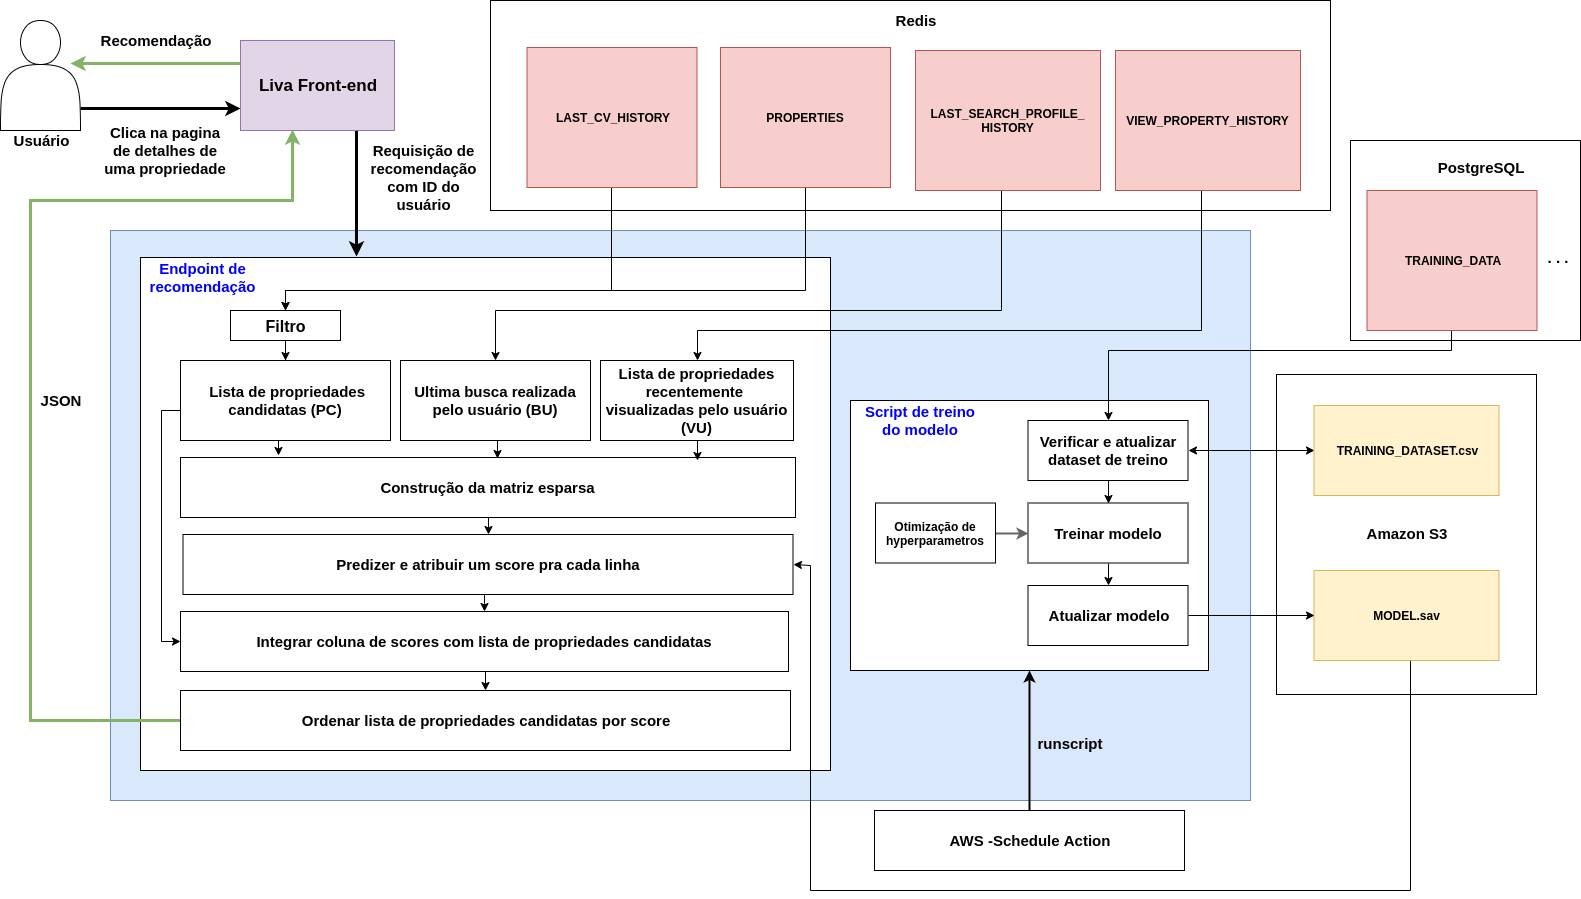
\includegraphics[scale=0.4]{figuras/proposta/sr_nivel3.png}
    \caption[Arquitetura do módulo de \textit{machine learning}]{Arquitetura do módulo de \textit{machine learning}. Fonte: Autor}
    \label{fig:sr_nivel3}
\end{sidewaysfigure}

Baseado na arquitetura acima, primeiramente é passado via requisição o ID do usuário para o \textit{endpoint} de recomendação, no momento em que um usuário entra na página de detalhes de uma propriedade, a fim de ser gerada as recomendações. Com o ID do usuário é possível recuperar os seguintes três tipos de variáveis:

\begin{itemize}
    \item \textbf{Última busca realizada pelo usuário (BU):} refere-se ao atual Perfil de Busca do usuário. Quando um usuário clica para visualizar uma propriedade, ela está sobre diversas condições de busca, como preço mínimo e máximo, tipo de imóvel, quantidade de quartos, dentre outras condições. Essas informações são guardadas na tabela LAST\_SEARCH\_PROFILE\_HISTORY;

    \item \textbf{Visualizações recentes em propriedades feitas pelo usuário (VU):} quando um usuário clica para visualizar os detalhes de uma propriedade. A cada clique é salvo um novo registro na tabela VIEW\_PROPERTY\_HISTORY. São salvos no máximo 100 registros dos últimos 3 meses para cada usuário. Esses registros são compostos de informações como preço, área, quantidade de quartos, dentre outras características de um imóvel;

    \item \textbf{Propriedade candidata a recomendação (PC):} refere-se às características da propriedade candidata a recomendação como preço, área, quantidade de quartos, dentre outras características. As propriedades são mantidas na tabela PROPERTIES.
\end{itemize}

Para a entrada do modelo de \textit{machine learning} existe um conjunto de {BU, VU, PC} e a saída é o score que reflete a probabilidade de CV, ou seja, a probabilidade de um usuário requisitar contato a um corretor de uma propriedade em específico.

\begin{equation}
    \{BU,VU,PC\}  \xrightarrow{F} \mathbb{R}
\end{equation}

Em que F é o modelo que atribui um score para um registro composto por BU, VU e PC. Um maior score significa maior chance de um CV. O \textit{dataset} de treino é composto por BU, VU e as características da propriedade de cada CV realizado ou descarte de uma propriedade do \textit{feed} referente a todos os usuários, ou seja, a variável alvo nesse caso é o CV, podendo ser 0 ou 1. O algoritmo de \textit{machine learning} vai construir um modelo capaz de distinguir entre CV = 1 e CV = 0 . No caso de um usuário descartar uma propriedade é considerado CV = 0.

A cada nova interação de descarte ou requisição de informação de uma propriedade os dados BU, VU e as características da propriedade em foco são salvos na tabela NEW\_TRAINING\_DATA. O treino é realizado por lotes agendados diariamente. Toda vez que o \textit{Script} de treino é executado, primeiramente, é verificado a existência de um arquivo .csv na Amazon S3 e em seguida é feita uma integração com os dados de treino da tabela. Logo em seguida é realizada a otimização de hiper-parâmetros com a técnica \textit{Grid Search}. O modelo é treinado e salvo como arquivo .sav na Amazon S3.

Toda vez que um usuário alcança a página de detalhes de uma propriedade é recuperado seu BU e VU e dessa forma é feito o score para cada candidato PC. Os candidatos são escolhidos baseados na mesma localidade da presente propriedade visualizada pelo usuário. Após realizado o score é feita uma ordenação dessas propriedades e em seguida são apresentadas as cinco primeiras ao usuário.

\begin{table}[H]
\centering
\begin{tabular}{ccccccc}
\hline
\textbf{\begin{tabular}[c]{@{}c@{}}Preço\\ máximo (BU)\end{tabular}} & \textbf{...} & \textbf{\begin{tabular}[c]{@{}c@{}}Quantidade\\ de\\ quartos 1\\ (VU)\end{tabular}} & \textbf{Preço 2 (VU)} & \textbf{\begin{tabular}[c]{@{}c@{}}Quantidade de\\ banheiro 2 (VU)\end{tabular}} & \textbf{...} & \textbf{CV} \\ \hline
400000 & ... & 1 & 150000 & 2 & ... & 1 \\ \hline
100000 & ... & 3 & null & null & ... & 0
\end{tabular}
\caption[Exemplo \textit{dataset} de treino]{Exemplo \textit{dataset} de treino. Fonte: Autor}
\end{table}

Para o presente problema de classificação foi escolhido o modelo de \textit{Gradient Boosting Decision Tree} (GBDT), discutido na seção \ref{machineLearning}. Como a característica do \textit{dataset} torna possível a existência de colunas com dados faltantes, é de grande importância a utilização de um método capaz de lidar com tal problema bem além de manter uma alta precisão. Por ser um modelo baseado em árvore de decisão, ele consegue lidar bem com atributos em seu valor bruto, o que é preferível em questões de manutenibilidade e performance pois não necessitará de pré-processamento. Além disso a tecnologia usada para o modelo lida naturalmente com dados faltantes. Segundo Synced (\citeyear{Synced:2017}) internamente, o XGBoost aprenderá automaticamente qual é a melhor direção a seguir quando um valor estiver faltando. Equivalentemente, isso pode ser visto como "aprender" automaticamente qual é o melhor valor de imputação para valores faltantes com base na minimização da perda do treinamento.

Os três tipos de variáveis apresentadas anteriormente, para entrada do modelo, são relacionadas a dois tipos matemáticos, numéricos e categóricos. Para os dados numéricos como preço ou quantidade de quartos, por exemplo, foi decidido manter seus valores em sua forma bruta, por questões de manutenibilidade e performance, para um processamento mais rápido. Para as variáveis categóricas, algumas colunas são excluídas, como o ID do usuário, que não é útil para a predição. A localidade será trocada pela sua latitude e longitude e o tipo de imóvel será trocado por variáveis fictícias binárias (0 e 1).

No Suumo.jp, Li et al. (\citeyear{Summo:2017}) encontra uma distribuição de tuplas no \textit{dataset} de treino entre CV = 1 e CV = 0, para cada uma linha com CV = 1 são gerada dez com CV = 0. Em seu modelo é proposto dez CV = 0 para dez propriedades aleatórias a cada um CV = 1. Dado que no modelo proposto para esse projeto temos a interação de descarte de uma propriedade, foi decidido não utilizar essa proporção e aleatoriedade pois isso fere com a  realidade dos dados dentro do contexto.

Li et al. (\citeyear{Summo:2017}) afirma que as variáveis categóricas devem ser tratadas em um modelo diferente das variáveis numéricas. Isso porque, como descrito anteriormente na seção \ref{machineLearning}, na construção da árvore de decisão como o algoritmo de ramificação se concentra na divisão de variáveis numéricas, a frequência de aparecimento de variáveis categóricas igualmente importantes para os usuários é relativamente reduzida, ou seja, as árvores de decisão vão favorecer as ramificações com variáveis numéricas. Dito isso Li et al. (\citeyear{Summo:2017}) propõe a separação de dois modelos, um somente com variáveis categóricas e o outro com numéricas. Para fazer a junçãhttps://pt.overleaf.com/project/5d707d197c21410001a0794bo dos scores gerados ele propõe a utilização de uma função de soma linear.

Como há uma quantidade muito pequena de características categóricas para o modelo proposto, não será feito a partição entre categóricas e numéricas.

\subsection{Sistema de recomendação baseado em crítica}

Com o intuito de não alterar o que já foi proposto no site da Liva, que faz o uso de uma ferramenta de busca baseada em preferência (Perfil de Busca) para recomendar propriedades, e ainda deixar o sistema de recomendação mais robusto seguindo uma abordagem, decidiu-se construir um sistema de recomendação baseado em crítica como descrito na seção \ref{Critiquing-based} seguindo a abordagem \textit{example critiquing}.
	
Segundo Burke, Felfernig e Goker (\citeyear{Burke}), e como já dito anteriormente, as abordagens tradicionais de recomendação, filtragem colaborativa e baseada em conteúdo, não são adequadas em situações de itens de alto valor, como propriedades ou veículos, que não são comprados com frequência. A abordagem baseada em conhecimento pode mitigar esse problema explorando requisitos explícitos do usuário, mas ela sofre de gargalos de aquisição de conhecimento associados aos esforços iniciais necessários para gerar o conhecimento do domínio.

Dessa forma a abordagem baseada em crítica surgiu para ser uma eficiente tecnologia de recomendação baseada na preferência do usuário e evitar os problemas descritos acima.

\subsubsection{Modelo da preferência}

Para o presente projeto decidiu-se por realizar a implementação da abordagem de \textit{example critiquing} melhorando a ferramenta de busca baseada em preferência já existente no site Liva. A ferramenta de busca baseada em preferências é utilizada para obter as preferências iniciais dos usuários, enquanto o \textit{example critiquing} é uma abordagem que permite aos usuários refinar suas preferências para localizar o item ideal que atenda às suas necessidades.

O usuário segue um processo como demonstrado na Figura \ref{fig:exemple-critiquing}:

\begin{figure}[H]
    \centering
    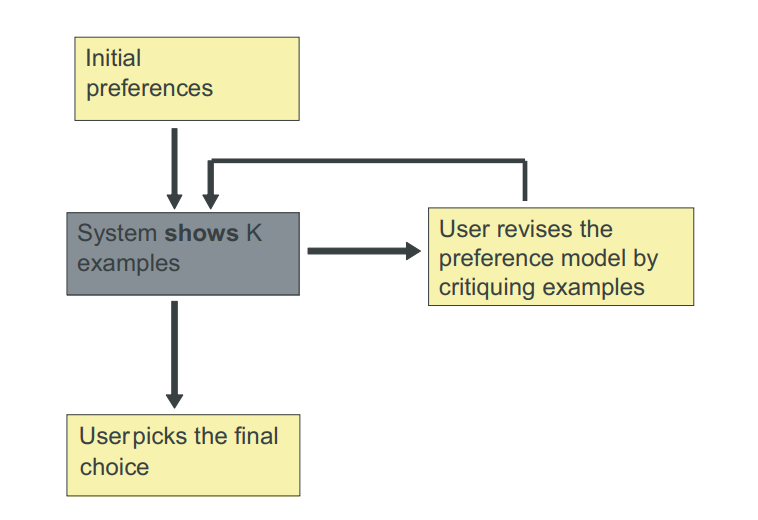
\includegraphics[scale=0.7]{figuras/proposta/exemple-critiquing.png}
    \caption[Interação Exemple-Critiquing]{Interação Exemple-Critiquing. Fonte: (Viappiani et al. 2006)}
    \label{fig:exemple-critiquing}
\end{figure}

Após o usuário ter definido seu modelo de preferência inicial o sistema é capaz de apresentar exemplos que o usuário possa considerar. Esses exemplos são propriedades que são ótimas para a atual busca de preferência (Perfil de Busca) configurada. O usuário irá revisar seu modelo de preferência através de críticas sobre os exemplos apresentados. Quando o usuário identifica o item certo, ele termina o processo.

O usuário irá apresentar suas preferências através do Perfil de Busca como na Figura \ref{fig:filtro_busca}. São comportados os seguintes atributos das propriedades: tipo de imóvel, faixa de preço, área, localização (Cidade e Bairro), quantidade de quartos, quantidade de suítes e quantidade de vagas na garagem. Além disso usuário seleciona a importância de cada atributo (peso de 1 a 5). O usuário irá criticar as propriedades de acordo com a Figura \ref{fig:prototipo_critico1}, em que ele pode postar críticas para a solução próxima, com as escolhas de manter ou melhorar algum atributo.

Como já demonstrado na seção \ref{Critiquing-based}, o modelo de preferência será baseado no MAUT (teoria da utilidade de atributos múltiplos) em que será computado a utilidade para cada propriedade e assim ordenadas e apresentadas.

Segundo Viappiani et al. (\citeyear{Viappiani}) no \textit{example critiquing}, cada crítica pode ser considerada como uma restrição leve, e o modelo de preferência pode ser desenvolvido simplesmente coletando críticas incrementalmente. Uma restrição leve é uma função de um atributo ou uma combinação de atributos para um número que indica o grau em que a restrição é violada.

Viappiani et al. (\citeyear{Viappiani}) dá o seguinte exemplo: um atributo que pode assumir os valores a, b e c, pode, para uma restrição leve, indicar preferência pelo valor b. Nesse caso haveria o mapeamento dos valores a e c para 1 e b para 0, indicando que somente b não quebrou a restrição. Uma preferência pela área de superfície de pelo menos 30 metros quadrados, onde uma pequena violação de até 5 metros quadrados pode ser aceitável, pode ser expressa por uma função linear por partes, como na Figura \ref{fig:funcao_linear}.

\begin{figure}[H]
    \centering
    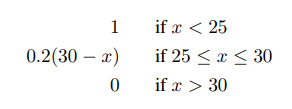
\includegraphics[scale=0.8]{figuras/proposta/funcao_linear.png}
    \caption[Função linear por partes]{Função linear por partes. Fonte: (VIAPPIANI, 2006)}
    \label{fig:funcao_linear}
\end{figure}

O autor considera que as restrições leves permitem que os usuários expressam preferências relativamente complexas de maneira intuitiva. Isso torna as restrições leves um forma útil para modelos de preferência de um \textit{example critiquing}.

\subsection{Banco de dados}

Como já descrito anteriormente serão utilizados dois tipos de banco de dados, um relacional com a tecnologia PostgreSQL e outro de valor-chave com Redis. Esses dois bancos são somente referente ao módulo de \textit{machine learning}, pois o módulo de crítica não necessita de armazenar dados.

Na base de dados relacional, serão armazenados dados para backup como o histórico de visualizações dos usuários (VIEW\_PROPERTY\_HISTORY), histórico de buscas realizadas pelo usuário (SEARCH\_PROFILE\_HISTORY) e as propriedades (PROPERTIES). Além disso são guardados dados de treino do modelo de \textit{machine learning} (TRAINING DATA).  Nas Figuras \ref{fig:der} e \ref{fig:diagrama_esquema} são apresentados os diagramas do banco de dados relacional.

\begin{figure}[H]
    \centering
    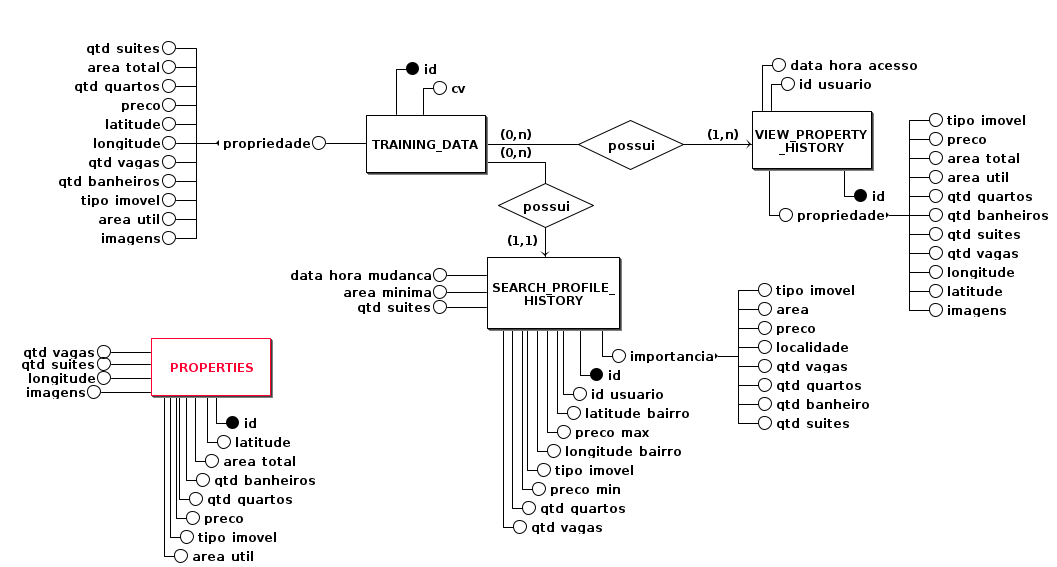
\includegraphics[scale=0.40]{figuras/proposta/der.png}
    \caption[Diagrama de Entidade-Relacionamento (DER)]{Diagrama de Entidade-Relacionamento (DER). Fonte: Autor}
    \label{fig:der}
\end{figure}

\begin{figure}[H]
    \centering
    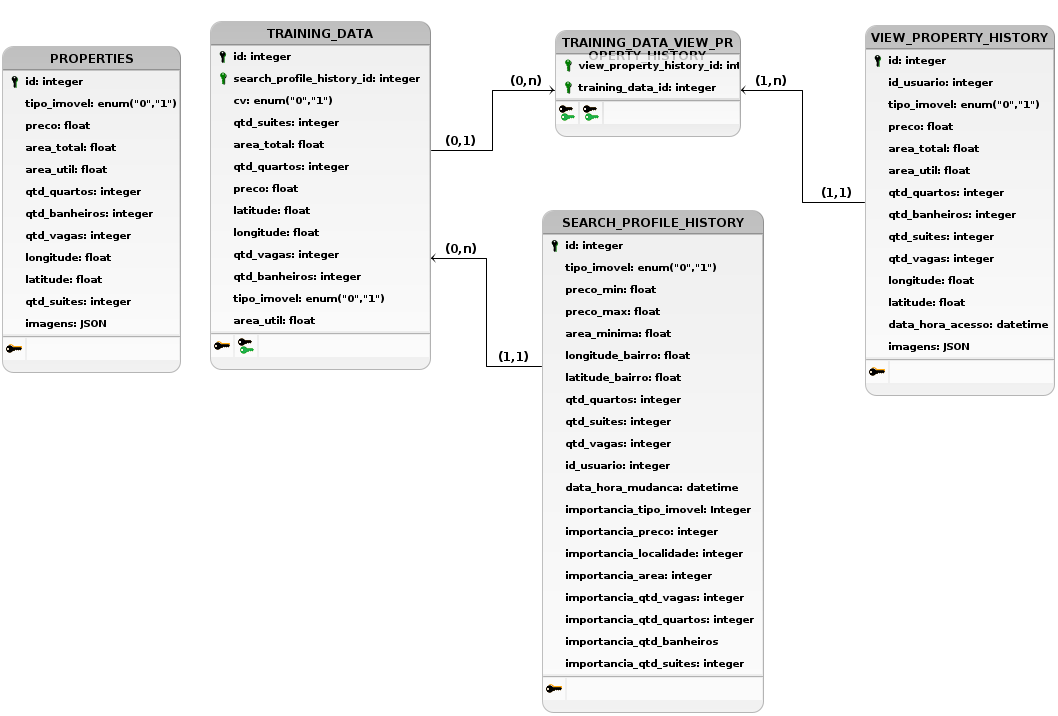
\includegraphics[scale=0.40]{figuras/proposta/diagrama_esquema.png}
    \caption[Diagrama de Esquemas]{Diagrama de Esquemas. Fonte: Autor}
    \label{fig:diagrama_esquema}
\end{figure}

Inicialmente a tabela SEARCH\_PROFILE\_HISTORY será populada com base nos perfis de buscas atuais dos usuários, adquiridos na base da dados da Liva. A tabela de propriedades em vermelho no diagrama da Figura \ref{fig:der}, está destacada dessa forma pois ela não será armazenada no banco do sistema de recomendação mas, como já existente, na base da Liva. No banco de dados da Liva as propriedades são atualizadas diariamente para cada imobiliária existente. Como os dados vindos de cada imobiliária não seguem um padrão e muitas vezes há a existência de muitas características faltantes, foi decidido focar somente em características comuns e raramente faltantes como: tipo do imóvel, área total e útil, preço, localidade, quantidade de quartos, banheiros e suítes.

A tabela dos dados de treino do modelo de \textit{machine learning} serão populadas com dados que serão coletados do início do semestre de 2020 até a conclusão do sistema em no final do mesmo ano, com o fim de se gerar um \textit{dataset} de treino inicial robusto.

Em relação ao banco de dados no Redis, como já apresentado na arquitetura anteriormente, existem quatro entidades como mostrado na Figura \ref{fig:redis}.

\begin{figure}[H]
    \centering
    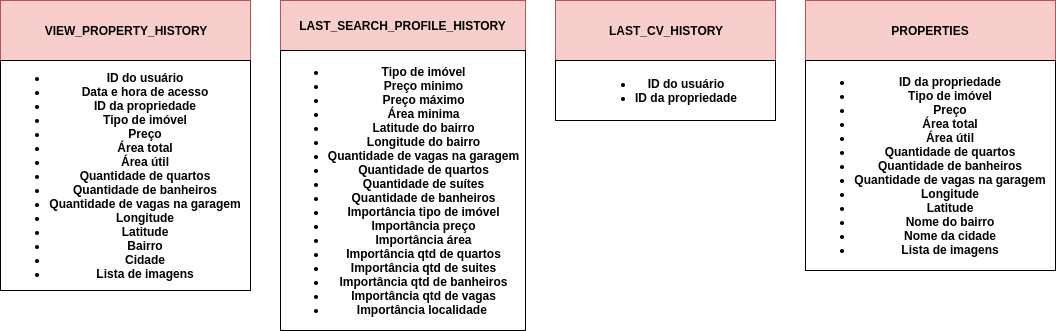
\includegraphics[scale=0.4]{figuras/proposta/redis.png}
    \caption[Representação do banco de dados no Redis]{Representação do banco de dados no Redis. Fonte: Autor}
    \label{fig:redis}
\end{figure}

Os dados da entidade PROPRIEDADES serão atualizados constantemente pelo serviço descrito na arquitetura, \textit{Data Updater}. Ele irá atualizar os dados a partir da leitura da tabela PROPERTIES concentrada no banco de dados da Liva.

\section{Suporte Tecnológico}

\subsection{Python}

Python é uma linguagem de programação de alto nível com o paradigma OO (orientada a objeto), sendo ela uma linguagem interpretada e não compilada, como por exemplo, a linguagem C. Conhecida também por ter uma sintaxe muito clara e exigir poucas linhas de código comparadas a outras linguagens de programação. Ela é altamente utilizada em vários serviços de grandes empresas. Dessa forma ela se faz uma linguagem formada por uma grande comunidade \cite{Python:2019}.

A versão que será implementada no serviço “Sistema de Recomendação API” é a 3.7.3.

\subsection{Django}

O Django é um \textit{framework} sob a licença BSD, criado para a linguagem python que usa o padrão MVT (\textit{Model-View-Template}), na qual é uma adaptação do clássico padrão MVC (\textit{Model-View-Controller}). Essa tecnologia visa o desenvolvimento rápido, pois é baseada no princípio  DRY (\textit{Don’t Repeat Yourself}), em que a ideia principal é evitar ao máximo retrabalho no desenvolvimento de software \cite{Django:2019}.

Ele também já cuida de várias rotinas comuns de aplicações \textit{Web}, como por exemplo: servidor, conexão com o banco de dados, organização de rotas (\textit{endpoints}), autenticação e entre outras rotinas. Contém também a tecnologia ORM (\textit{Object-relational mapping}), que tem o intuito de mapear cada atributo e relacionamento das classes para o banco de dados, ou seja, não é necessário criar \textit{scripts} SQL (\textit{Structured Query Language}) na mão para tal. 

A versão que será usada no projeto para o serviço “Sistema de Recomendação API” é a 2.2.

\subsection{Django REST \textit{Framework}}

Para construção da API (\textit{Application Programming Interface}) com o paradigma arquitetural REST será utilizado a ferramenta denominada Django REST \textit{framework} que disponibiliza diversas ferramentas para construção da mesma, sendo que ela ainda possibilita algumas funcionalidades extras, como o \textit{serializer}, que permite a conversão de tipos de dado como JSON e XML para os tipos de dados nativos do python, e vice e versa \cite{DjangoRest:2019}.

A respeito dessa ferramenta, ela usa o padrão MV (\textit{Model-View}), pois por ser uma API, não há o \textit{Template} que teria o papel de um \textit{front-end}, como no Django. Essa tecnologia também possui uma grande comunidade, excelente documentação para consulta e é altamente utilizada por grandes empresas, como:  Mozilla , Red Hat , Heroku e Eventbrite \cite{DjangoRest:2019}.

A versão que será usada para implementação do serviço “Sistema de Recomendação API” será a 3.10.3.

\subsection{Scikit-Learn}

O Scikit-Learn é um módulo do python que possui vários algoritmos de aprendizagem de máquina (por exemplo \textit{random forest e gradient boosting}) para problemas supervisionados e não supervisionados. Está biblioteca é construída em Numpy e Scipy e tem como objetivo trazer conhecimento de \textit{machine learning} para os usuários não especialistas usando uma linguagem de alto nível (python). Um dos destaques dessa tecnologia está na facilidade de uso, no desempenho e na documentação \cite{PREDEGOSA:2011}.

A versão que será usada para implementação será a 0.21.3.

\subsection{Pandas}

Pandas é uma biblioteca do python de código aberto com a licença BSD, que preza em um bom desempenho e facilidade de uso. O propósito deste módulo é realizar análise e modelagem de dados (bem parecido com a linguagem R) usando o objeto conhecido como “\textit{DataFrame}”, podendo ler e escrever dados no formato CSV (\textit{Comma-Separated-Values}), texto, SQL (\textit{Structured Query Language}), HDF5 e Excel \cite{pandas:2019}.

A versão que será usada para implementação será a 0.3.1.

\subsection{Numpy}

Numpy é um pacote fundamental do python com a licença BSD (Berkeley \textit{Software Distribution}) quando se trata de \textit{Data Science} (ciência de dados) que adiciona um poderoso objeto com matriz N-dimensional, podendo integrar com código C, C++ e Fortran. Além de ter recursos importantes de álgebra linear (transformação de Fourier, números aleatórios, por exemplo) \cite{numpy:2019}.

A versão que será usada para implementação será a 1.17.3.

\subsection{Pickle}

O Pickle é um módulo do python que implementa protocolos binários com a finalidade de serializar e desserializar uma estrutura de objetos dessa mesma linguagem. O “\textit{Pickling}” significa transformar um objeto da hierarquia do python para fluxo em bytes, já o (desserializar) é o fluxo contrário a isso \cite{pickle:2019}.

A versão que será usada para implementação será a 5.

\subsection{Xgboost}

Xgboost é uma \textit{library} de licença Apache que proporciona o \textit{gradient boosting} com suporte para C++, Python, R e outras linguagens de programação. Criada para ser altamente eficiente, flexível e portátil, resolvendo vários problemas de ciência de dados utilizando algoritmos de \textit{machine learning} sob a estrutura \textit{gradient boosting} \cite{XGBOOST:2019}.

A versão que será utilizada no serviço “Sistema de Recomendação API” será a 0.90.

\subsection{JavaScript}

JavaScript é uma linguagem de programação interpretada (assim como o python) muito utilizada no lado do cliente, mas também podendo ser usado do lado do servidor para tratamento de dados. Sendo a linguagem mais usada atualmente no lado do cliente, ou seja, no navegador do usuário, juntamente com HTML5 e CSS3, deixando as páginas Web estáticas, agora interativas. Com o avanço da linguagem e a criação do \textit{framework} NodeJS, atualmente JavaScript é muito usado no \textit{back-end} dos serviços \cite{JavaScript:2019}.

A versão que será utilizada para a implementação dos serviços “Data Updater” será a EcmaScript 6.

\subsection{NodeJS}

O NodeJS é definido como um “ambiente de execução Javascript do lado do servidor”, ou seja, é um framework orientado a eventos baseado na linguagem Javascript que possibilita a criação de aplicações não dependentes de um navegador. Um ponto positivo que levou a sua alta adoção pelos programadores é a sua alta escalabilidade, além de sua arquitetura flexível e sendo um ótimo aliado a arquitetura de microsserviços \cite{nodejs:2019}.

Um dos diferenciais do NodeJS é o gerenciador de pacotes que ele tem, o NPM, que contém o maior repositório de software do mundo, sendo que um dos pacotes é o Express, na qual é um framework para desenvolvimento \textit{Web} \cite{lenon:2018}.

A versão que será utilizada para a implementação do serviço “Data Updater” será a 13.1.0.

\subsection{ReactJS}

ReactJS é um biblioteca Javascript orientada a componentes que tem como objetivo criar interfaces interativas de usuário sem muita complexidade. Cada componente tem seu próprio estado chamado de “\textit{state}” e a cada mudança desse estado, o React atualiza e renderiza quase instantaneamente aquele componente. Essa tecnologia é compatível com a sintaxe JSX, mas sendo opcional e não obrigatório seu uso pelo programador \cite{reactjs:2019}.

A versão já utilizada no serviço de \textit{front-end} da Liva e que também será utilizada para implementação dos novos componentes do sistema de recomendação será a 16.11.

\subsection{Bootstrap}

Bootstrap é uma ferramenta de código livre para desenvolvimento de sites e aplicativos web que tem HTML, CSS e JavaScript. Sendo um dos \textit{frameworks} mais famosos do mundo usado para criar sites responsivos e mobile, disponibilizando componentes Web com estilos prontos e \textit{templates} de \textit{sites} \cite{bootstrap:2019}.

A versão já usada no serviço de \textit{front-end} da Liva e que também será utilizada para implementação dos novos componentes do sistema de recomendação será a 4.3.

\subsection{Ruby}

Ruby é uma linguagem de programação de código totalmente livre orientada a objeto, tal qual que tudo em ruby é objeto, pois cada parte do código tem suas propriedades e ações relacionadas a aquele tipo de objeto. O Ruby também é flexível, ou seja, os utilizadores podem remover e redefinir partes da linguagem a vontade. Além disso, o Ruby usa o padrão “\textit{sugar syntax}” (açúcar sintático) que facilita lembrar de como escrever o código \cite{ruby:2019}.

A versão já usada no serviço \textit{back-end} “Liva API” é a 2.6.5.

\subsection{Rails}

Rails é um meta-framework (um framework compostos de outros frameworks) feito com a linguagem Ruby e também é de código aberto sob a licença MIT, assim como a própria linguagem. O padrão arquitetural seguido por essa tecnologia é o clássico MVC (Model-View-Controller), e também os padrões Web, como JSON e XML. A idéia principal do Rails é aumentar a velocidade e facilidade de criar uma aplicação Web \cite{portalgsti:2019}.

A versão já usada no serviço \textit{back-end} “Liva API” é a 6.0.1.

\subsection{PostgreSQL}

PostgreSQL é uma famoso banco relacional de código aberto que usa a linguagem de \textit{script} SQL. Ele também contém vários recursos para a escala e a segurança das cargas de trabalho de dados. Esse banco ganhou sua reputação através da sua arquitetura robusta, confiabilidade, integridade, um conjunto de recursos e a dedicação de sua comunidade. Atualmente, ele é o banco relacional de código aberto preferido pelos desenvolvedores \cite{postgres:2019}.
Fora essas características, o PostgreSQL é altamente extensível, no sentindo do desenvolvedor poder criar seus próprios tipos de dados e funções personalizadas \cite{postgres:2019}.

A versão que já está sendo usada como banco de dados para o serviço “Liva API” e que será usado nos outros banco de dados será á 12.0.

\subsection{Redis}

O Redis é uma base de dados em memória com licença BSD, ou seja, tem código aberto. Muito utilizado como cache e banco de dados em serviços, suportando vários tipos de dados, como: \textit{strings, hashes, lists, sets, sorted sets} dentre outros. Ele permite realizar algumas operações atômicas com os dados, por exemplo, inserir em uma \textit{string}, incrementar algum valor numa \textit{hash}, inserir elementos numa \textit{list} e outros operações \cite{redis:2019}.

O responsável pelo seu excelente desempenho é o conjunto de dados na memória, mas caso seja necessário é capaz de gravar em disco ou anexar informações em \textit{log} \cite{redis:2019}.

A versão que será utilizada para se conectar com o serviço “\textit{Data Updater}” e o “Sistema de Recomendação API” é a 5.0.

\subsection{Docker}

Docker é uma ferramenta de virtualização muito usada em vários serviços, na qual foi projetada para facilitar a criação e a implantação usando os chamados “contêineres” de modo que cada \textit{container} pode ser feito um empacotamento de algum determinado serviço com todos os pacotes e configurações necessárias para a execução dele \cite{OPENSOURCE.COM:2019}.

O Docker disponibiliza uma grande quantidade de imagens no repositório chamado DockerHub, sejam elas oficiais ou feitas por desenvolvedores ao redor do mundo. Essas imagens contém Linux, possibilitando a base para criação da virtualização da aplicação \cite{DOCKERHUB:2019}.

A versão que será usada para virtualização dos serviços “\textit{Data Updater}” e “Sistema de Recomendação API” é a 19.03.

\subsection{Amazon \textit{Elastic Container Service}}

O Amazon ECS como é conhecido, é uma plataforma de gerenciamento de contêineres rápida e dimensível que possibilita o gerenciamento de contêineres dentro de um \textit{cluster}. O usuário é capaz de iniciar ou parar aplicações que rodam nesses contêineres com um simples comando, inclusive disponibiliza o estado de cada serviço rodando dentro do \textit{cluster} \cite{amazonECS:2019}.

Ele dá a possibilidade do usuário escolher os recursos que deseja para rodar determinado serviço e sem se preocupar com as configurações de cada recurso ou com a escalabilidade da infraestrutura de gerenciamento \cite{amazonECS:2019}.

\subsection{Amazon Kinesis}

O Amazon Kinesis é um serviço que serve para coleta, análise e transmissão (\textit{streaming}) de grandes quantidades de dados em tempo real. O Kinesis pode ser executado em instâncias do Amazon EC2 com a biblioteca Kinesis Client. Essa tecnologia possibilita enviar os dados processados para vários outros serviços AWS \cite{KINESIS:2019}.

\subsection{Amazon S3}

O  Amazon Simple Storage Service (Amazon S3) é um serviço de armazenamento de dados junto com escalabilidade, durabilidade, segurança e performance, ou seja, é possível armazenar qualquer volume de dados em uma grande escala de variabilidade. O gerenciamento e a organização dos dados é feito de maneira fácil \cite{S3:2019}.

\subsection{Git}

Git é uma ferramenta de código aberto de controle de versão planejado para pequenos até grandes projetos com rapidez. O seu diferencial comparado a outras ferramentas de versionamento é a sua estrutura de \textit{branches} (ramificações) e \textit{mergings} (fundição), na qual é possível criar várias \textit{branches} locais totalmente independentes uma da outra, além da criação e da exclusão ser fácil e rápida \cite{git:2019}.

A versão que será usada nos serviços “\textit{Data Updater}” e “Sistema de Recomendação API” será a 2.24.

\subsection{Github}

Github é um repositório de código com o controle de versionamento Git. Essa plataforma possibilita que os usuários contribuam em projetos privados ou abertos. Sendo altamente usado no mundo todo  por programadores, tanto para armazenar seus projetos, quanto para divulgar seu portfólio profissional com seus projetos. Também contém ótimos meios de comunicação para relatar dúvidas, erros e requisitar mudanças em algum projeto. Atualmente o Github contém por volta de 100 milhões de repositórios de código hospedado \cite{github:2019}.

\subsection{Zenhub}

Zenhub é uma ferramenta de gerenciamento de projetos ágeis para desenvolvedores de software integrado a plataforma do GitHub. Usando as informações do projeto trazidas do próprio GitHub, essa ferramenta é capaz de gerar gráficos, relatórios, fluxo de trabalho dos desenvolvedores e andamento do projeto \cite{zenhub:2019}.

\subsection{LáteX}

Látex é um sistema de preparação de documentos para tipografia, sendo mais utilizado em documentos científicos e técnicos, mas podendo ser usado em outros tipos de documento que o usuário deseja publicar. Esse sistema incentiva o autor a se preocupar com o conteúdo do documento e não com sua aparência \cite{latex:2019}.

\subsection{Overleaf}

O Overleaf tem o objetivo de resolver os problemas ao escrever em Látex, ou seja, torná-lo mais acessível para cientistas e escritores técnicos em todas as etapas. Disponibilizando um visualizador de LáteX que já converte para PDF, além disso, essa plataforma salva seus documentos em nuvem, tendo assim, mais segurança e permite uso grátis para estudantes \cite{overleaf:2019}.

\section{Simulação}

Com o fim de validar a aplicabilidade da proposta, foi desenvolvido um protótipo (Apêndice \ref{apendice}) da solução proposta. Para o desenvolvimento desse protótipo, como a solução se baseia em duas abordagens diferentes (módulo de critica e módulo de \textit{machine learning}), foi decidido fazer a implementação das duas de forma reduzida e minimalista. De forma geral, para o recomendador baseado em critica, é disponibilizado para o usuário uma pergunta que servirá para criticar apenas uma característica do imóvel, como apresentado nas Figuras \ref{fig:prototipo_simulacao_critica1}, \ref{fig:prototipo_simulacao_critica2} e \ref{fig:prototipo_simulacao_critica3}.


\begin{figure}[H]
    \centering
    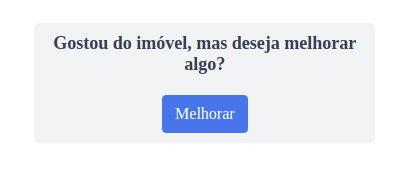
\includegraphics[scale=0.9]{figuras/consideracoes_finais/prototipo_simulacao_critica1.jpg}
    \caption[Protótipo da simulação da crítica parte 1]{Protótipo da simulação da crítica parte 1. Fonte: Autor}
    \label{fig:prototipo_simulacao_critica1}
\end{figure}

\begin{figure}[H]
    \centering
    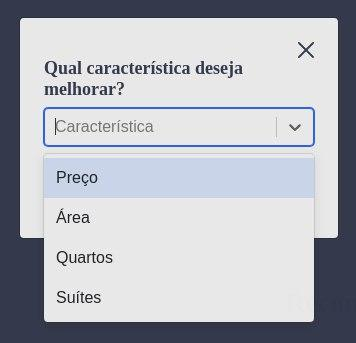
\includegraphics[scale=0.7]{figuras/consideracoes_finais/prototipo_simulacao_critica2.jpg}
    \caption[Protótipo da simulação da crítica parte 2]{Protótipo da simulação da crítica parte 2. Fonte: Autor}
    \label{fig:prototipo_simulacao_critica2}
\end{figure}

\begin{figure}[H]
    \centering
    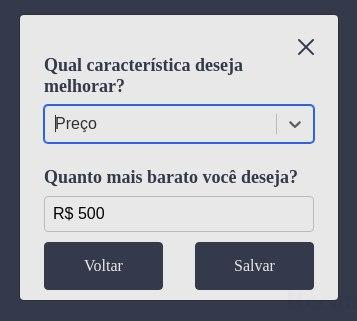
\includegraphics[scale=0.7]{figuras/consideracoes_finais/prototipo_simulacao_critica3.jpg}
    \caption[Protótipo da simulação da crítica parte 3]{Protótipo da simulação da crítica parte 3. Fonte: Autor}
    \label{fig:prototipo_simulacao_critica3}
\end{figure}

Dessa forma o usuário selecionará uma das características e atribuirá o valor de sua preferencia. Em seguida o perfil de busca do usuário será refinado baseado na critica dessa característica em si, e assim serão geradas novas recomendações em seu \textit{feed}.

No recomendador de \textit{machine learning} foi decidido a construção de um \textit{collaborative filtering} baseado em modelo, utilizando-se da técnica de fatoração matricial, com o algoritmo de \textit{machine learning} \textit{Non-negative matrix factorization} (NMF) disponibilizado pela biblioteca sklearn. Para simular a integração do sistema de recomendação como um serviço, foi construída uma API própria para o protótipo. Seu \textit{deploy} foi feito por meio do serviço ECS do AWS, e tem um banco de dados próprio.Os dados de entrada do modelo foram retirados do banco de dados da Liva. Esses dados são referentes as ações de "Favoritar" e "Descartar" um imóvel feitas pelos usuários e foram copiados para o banco de dados da API.

Os dados dos usuários serão atualizados assim como modelo será treinado diariamente. A transformação da matriz que terá todos os usuário e todos os imóveis "avaliados", disponibilizará um \textit{score} (pontuação) para cada propriedade. Dessa forma será possível recomendar para todos os usuários as cinco melhores propriedades geradas pelo algorítimo. Essas recomendações são apresentadas na página de detalhes do imóvel, assim como na solução proposta, e por meio de um componente carrossel do ReactJS chamado "\textit{swiper}" como na Figura \ref{fig:prototipo_simulacao_rs}.

\begin{figure}[H]
    \centering
    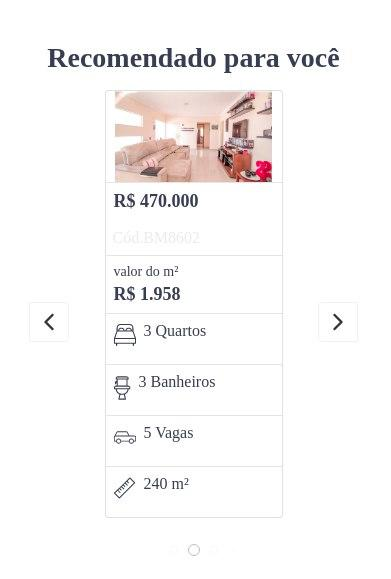
\includegraphics[scale=0.6]{figuras/consideracoes_finais/prototipo_simulacao_rs.jpg}
    \caption[Protótipo do sistema de recomendação]{Protótipo do sistema de recomendação. Fonte: Autor}
    \label{fig:prototipo_simulacao_rs}
\end{figure}

Foram obtidos dados por meio da ferramenta Mixpanel em integração com o \textit{Front-end} da Liva. Esses dados referem-se a consultas realizadas pelo usuário dado um período de tempo. São registradas a frequência de acesso ao \textit{feed}, visualização a pagina de detalhes, edição do perfil de busca, avaliação (favoritar ou descartar) de um imóvel, solicitação de mais imóveis a serem recomendados no \textit{feed}, alteração de ação de favoritar ou descartar imóvel dentre outros. Além disso, foram separados todas as recomendações feitas para os usuários do banco da Liva.

O protótipo ficou em produção do dia 26 ao dia 27 de novembro. Assim o resultado obtido foi comparado com os dois dias da semana anterior (19 e 20 de novembro). Abaixo se encontra a representação dos dados obtidos.


\begin{table}[H]
\centering
\begin{tabular}{lcc}
\hline
\textbf{Data do inicio - Data do fim} & 19/11/19 - 20/11/19 & 26/11/19 - 27/11/19 \\ \hline
\textbf{Quantidade de recomendações} & 715 & 537 \\ \hline
\textbf{Quantidade de imóveis favoritados} & 0 & 6 \\ \hline
\textbf{Quantidade de imóveis descartados} & 19 & 7 \\ \hline
\end{tabular}
\caption[Quantidade de recomendações, imóveis favoritados e descartados]{Quantidade de recomendações, imóveis favoritados e descartados. Fonte: Autor}
\label{tab:my-table}
\end{table}

% 421 - recomendações
% 6 - likes
% 3 - dislikes
% 1.42

% 1055 - recomendações
% 10 - likes
% 12 - dislikes
% 0.94

\subsection{Analise dos resultados}

Com os dados obtidos foi possível analisar a aprovação das recomendações, medindo o grau de imoveis favoritados, dividindo o numero de imoveis recomendados favoritados pelo numero total de recomendações multiplicado por 100, e o grau de imoveis descartados com o numero de imóveis descartados, como apresentado na tabela abaixo.

\begin{table}[H]
\centering
\begin{tabular}{lcc}
\hline
\textbf{Data do inicio - Data do fim} & 24 /11/19 - 25/11/19 & 26/11/19 - 27/11/19 \\ \hline
\textbf{Grau de imóveis favoritados} & 0.0 & 1.11 \\ \hline
\textbf{Grau de imóveis descartados} & 2.65 & 1.30 \\ \hline
\end{tabular}
\caption[Grau de imóveis favoritados e descartados]{Grau de imóveis favoritados e descartados. Fonte: Autor}
\label{tab:my-table2}
\end{table}

Com isso é possível perceber uma melhora do grau de imoveis favoritados durante o período com a aplicação dos dois recomendadores com abordagens, além de apresentar uma menor taxa de descartes.